\section*{PCIe 6.0 CTLE Specifications}
\label{ch:specs}

\section*{PCIe 6.0 Equalization Requirements}
The evolution of peripheral component interconnects to the PCIe 6.0 standard introduces a target data rate of 64.0 GT/s. At these extremely high transmission speeds, signals traveling over copper traces experience severe, frequency-dependent insertion loss. This attenuation disproportionately degrades the high-frequency components of the transmitted signal, leading to severe Inter-Symbol Interference (ISI) at the receiver. To reliably recover the data and maintain the required Bit Error Rate (BER), robust equalization is critical. Consequently, the PCIe 6.0 specification mandates the use of a high-order behavioral Continuous-Time Linear Equalizer (CTLE) within the reference receiver model. 

The primary function of this CTLE is to provide high-frequency peaking that operates inversely to the channel's insertion loss profile. By carefully tuning the CTLE transfer function, the overall system response (Channel + CTLE) is flattened across the Nyquist bandwidth, significantly opening the received data eye prior to further digital equalization stages such as Decision Feedback Equalization (DFE).

\newpage
\section*{Behavioral CTLE Specifications}
To achieve the shaping flexibility necessary to compensate for a wide variety of standard channel models, the behavioral CTLE defined for the 64.0 GT/s data rate consists of a complex transfer function featuring six poles and three zeros. This is typically modeled as a series of cascaded stages to achieve the required high-order shaping, as illustrated in Figure~\ref{fig:behav_model_stages}.

\begin{figure}[H]
    \centering
    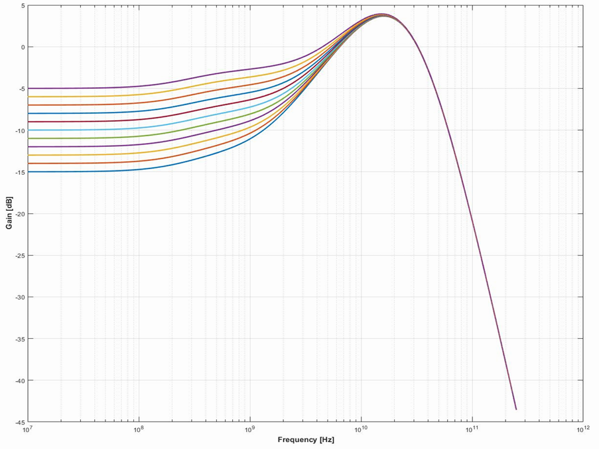
\includegraphics[width=\textwidth]{img/CTLE_img/pcie6_standard_extracted_behav_model_ctle.png}
    \caption{Cascaded CTLE stages extracted from the PCIe 6.0 standard behavioral model.}
    \label{fig:behav_model_stages}
\end{figure}

\noindent A critical component of this behavioral model is its highly adjustable DC gain parameter. The standard specifies strict boundaries and granularities for this tuning to ensure reliable compensation across different physical routing environments. 

\newpage \noindent The target specifications extracted from the PCIe 6.0 standard, which serve as foundational design constraints throughout this work, are provided in Figure~\ref{fig:ctle_spec_img} and summarized in Table~\ref{tab:specs}.

\begin{figure}[H]
    \centering
    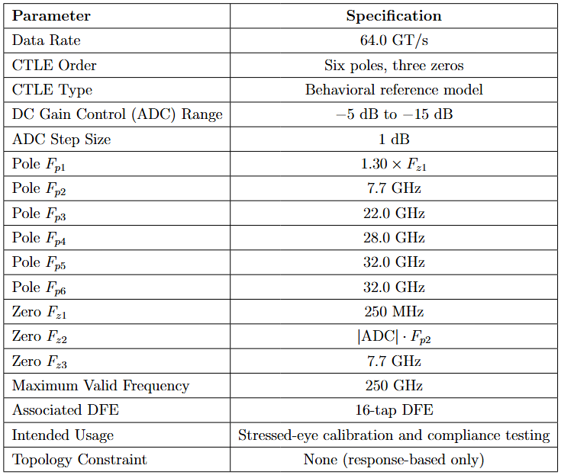
\includegraphics[width=0.8\textwidth]{img/CTLE_img//pcie6_standard_ctle_spec.png}
    \caption{Target CTLE specifications extracted from the PCIe 6.0 standard.}
    \label{fig:ctle_spec_img}
\end{figure}

\begin{table}[H]
    \centering
    \caption{Summary of the CTLE design specs extracted from the PCIe 6.0 standard.}
    \label{tab:specs}
    \renewcommand{\arraystretch}{1.2}
    \begin{tabular}{@{}lcc@{}}
        \toprule
        \textbf{Parameter}    & \textbf{Specification}       & \textbf{Unit} \\
        \midrule
        Supply voltage        & $0.8 \pm 5\%$    & V             \\
        Data rate             & 64               & Gb/s          \\
        DC gain range         & $-5$ to $-15$    & dB            \\
        DC gain step size     & 1                & dB            \\
        Maximum HF boost      & 19               & dB            \\
        Current consumption     & $< 20$           & mA            \\
        Temperature range     & $-40$ to $+120$  & \si{\celsius} \\
        \bottomrule
    \end{tabular}
\end{table}

\noindent The maximum high-frequency boost of 19 dB is essential for deep-insertion-loss channels, while the 1 dB step size allows the receiver adaptation algorithms to finely tune the equalization profile without over-amplifying high-frequency noise or crosstalk.

\section*{Channel Model Characteristics and Test Setup}
Validating the behavioral model requires a robust transient and AC simulation environment. The channel model dictates the baseline amount of equalization required. For this testbench, the physical channel was constructed by cascading a fundamental 1-inch FR4 segment, illustrated in Figure~\ref{fig:channel_model}. 

\begin{figure}[H]
    \centering
    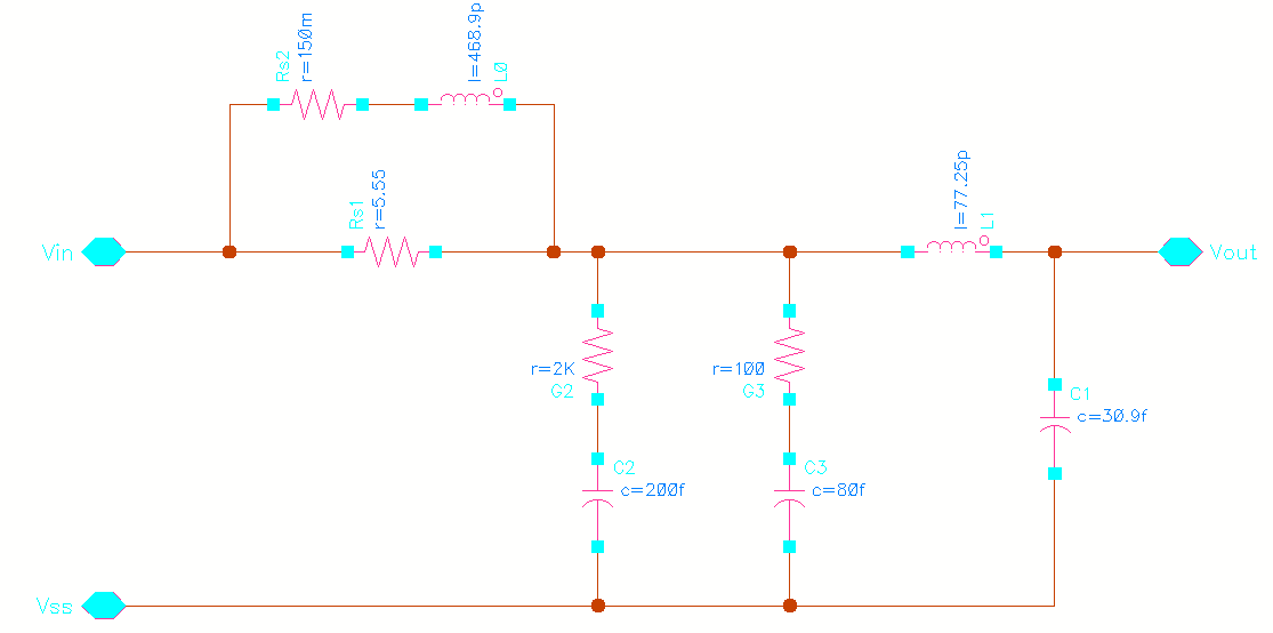
\includegraphics[width=0.8\textwidth]{img/CTLE_img/channel_model.png}
    \caption{The 1-inch FR4 segment used as the fundamental building block to construct the physical channel model.}
    \label{fig:channel_model}
\end{figure}

\noindent This cascaded configuration results in a severe channel model exhibiting an insertion loss of approximately $-$26 dB at the Nyquist frequency. This deep-loss profile is utilized to strictly evaluate the CTLE's compensation limits.

\begin{figure}[H]
    \centering
    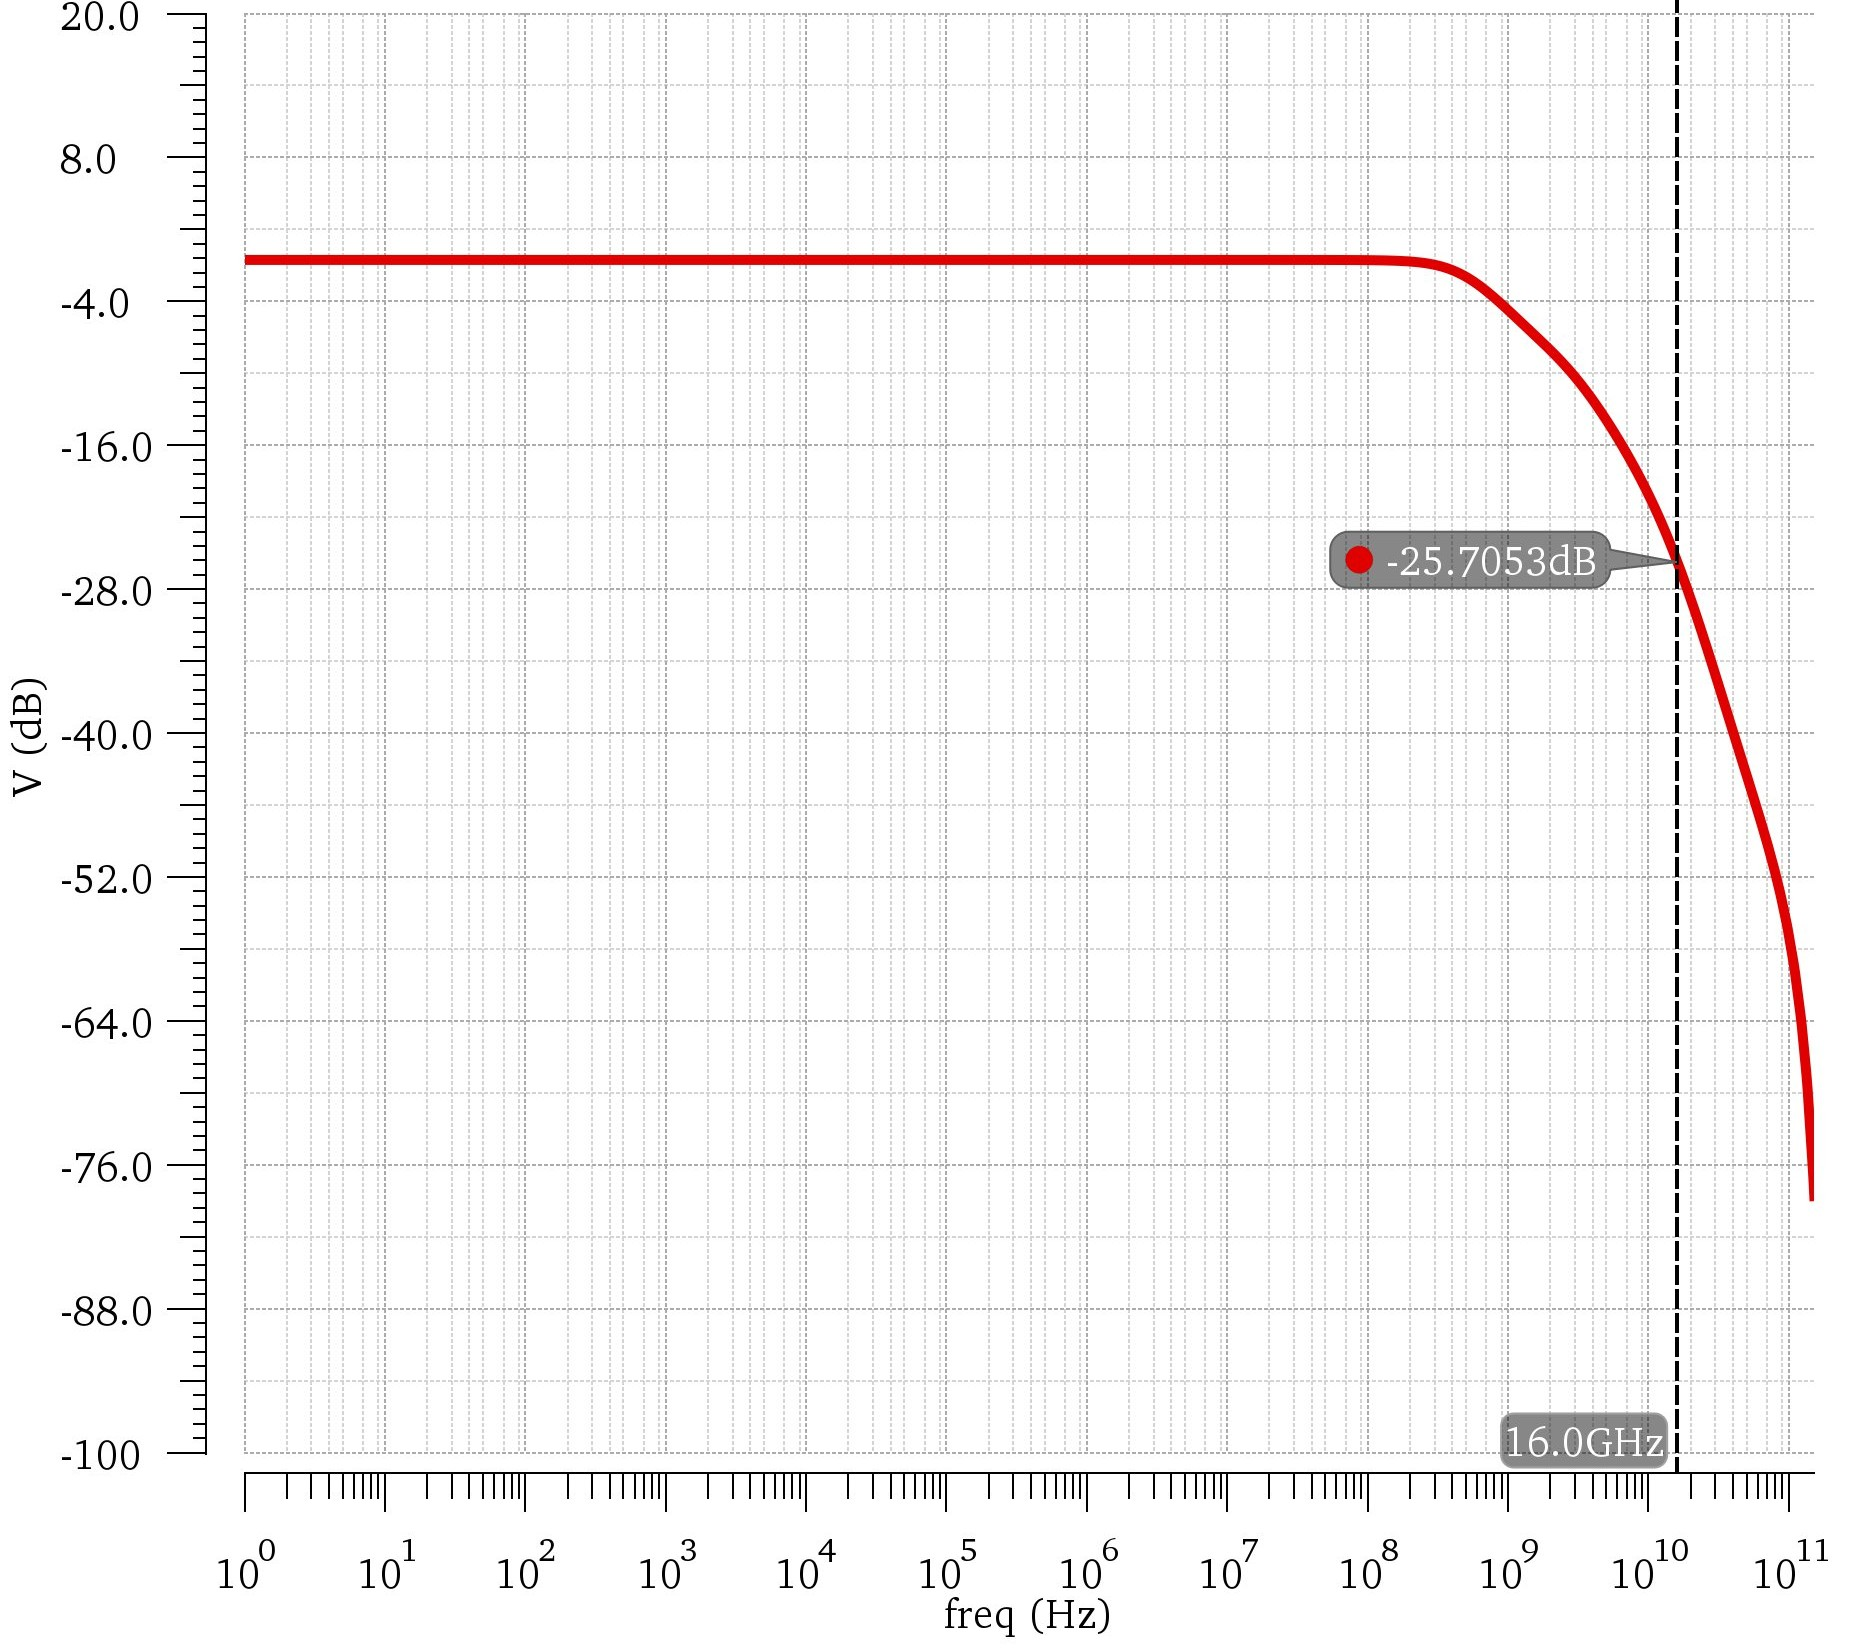
\includegraphics[width=0.65\textwidth]{img/CTLE_img/channel_response.jpg}
    \caption{Frequency response of the cascaded channel model, illustrating a severe insertion loss of approximately $-$26 dB at the Nyquist frequency.}
    \label{fig:channel_response}
\end{figure}

\noindent Before implementing the transistor-level design, \textbf{the behavioral CTLE was implemented in Verilog-A code}. Behavioral simulations were then conducted to observe the AC response of the CTLE and its interaction with this uncompensated $-$26 dB channel. Figure~\ref{fig:behavioral_ctle_curves} demonstrates the AC response of the behavioral model, sweeping through its various adjustable DC gain configurations to provide different levels of peaking.

\begin{figure}[H]
    \centering
    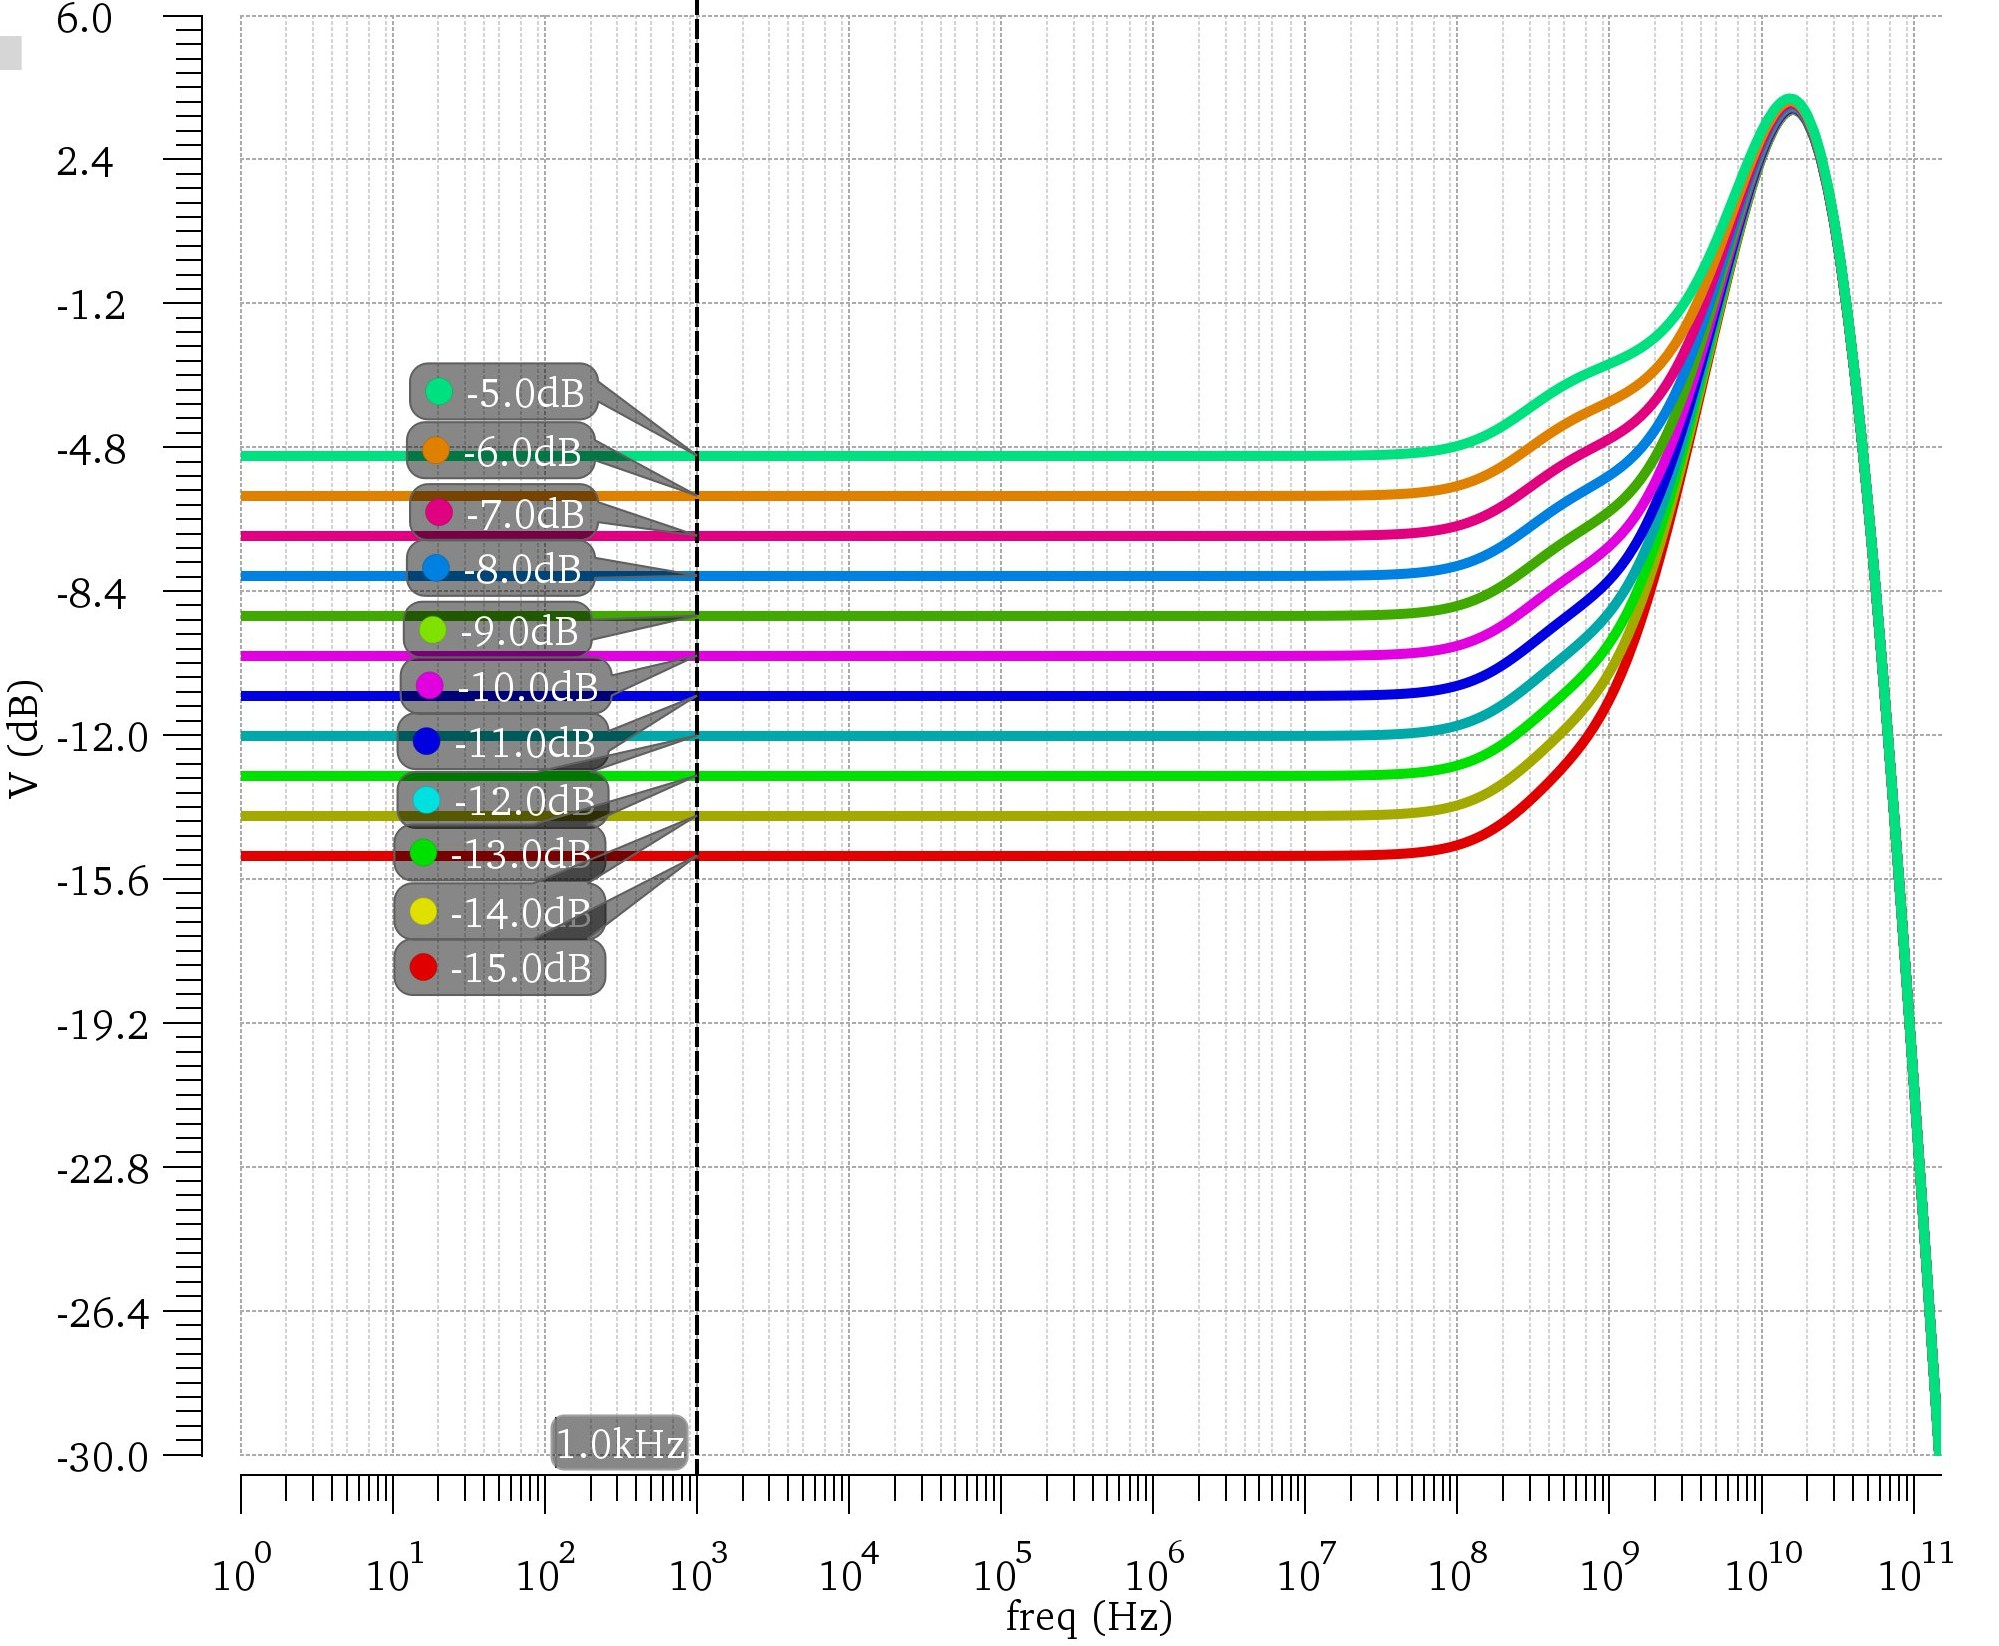
\includegraphics[width=0.85\textwidth]{img/CTLE_img/behavioral_ctle_response.jpg}
    \caption{Behavioral CTLE simulation showing the AC response curves across various DC gain configurations.}
    \label{fig:behavioral_ctle_curves}
\end{figure}

\noindent The simulation setup utilizes a Pseudorandom Binary Sequence (PRBS). For the behavioral tests, an Linear Feedback Shift Register (LFSR) mode of PN13 was utilized as the primary stimulus. The bit period is defined as 1 Unit Interval (UI), and realistic signal transitions were modeled with both rise time and fall time configured to 0.1 UI.\\

\noindent By tuning the CTLE's DC gain and zero locations, the high-frequency peaking is configured to invert the channel's $-$26 dB attenuation profile. When this equalization is mathematically superimposed over the channel response, the resulting total transfer function demonstrates a significantly flattened magnitude across the frequency band of interest, successfully verifying the theoretical limits of the 6-pole, 3-zero model.

\section*{Transient Simulation and PAM4 Eye Recovery}
Because PCIe 6.0 utilizes Pulse Amplitude Modulation 4-level (PAM4) signaling to achieve the 64 GT/s data rate, the equalizer must clearly resolve three distinct data eyes. Signal integrity is measured by evaluating these eye openings post-equalization.

\begin{figure}[H]
    \centering
    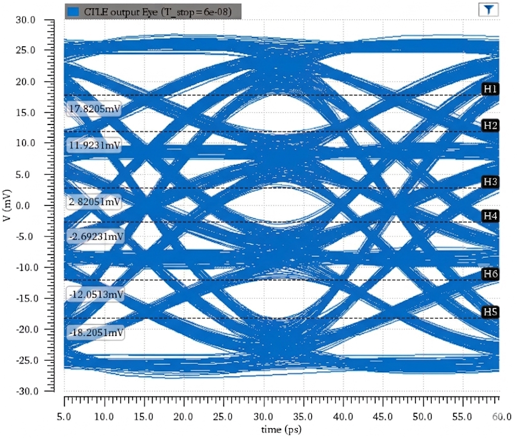
\includegraphics[width=0.85\textwidth]{img/CTLE_img/behavioral_CTLE_AC_eye_diagram_19db_channel.png}
    \caption{Post-CTLE Behavioral Eye Diagram at 64 GT/s. The equalization successfully recovers the three distinct PAM4 eyes after passing through the physical channel.}
    \label{fig:eye_diagram}
\end{figure}

\noindent Figure~\ref{fig:eye_diagram} presents the CTLE output eye diagram captured during the transient simulation. The effectiveness of the behavioral model is evidenced by the distinct separation of the PAM4 levels despite the severe channel attenuation. The eye diagram explicitly maps the critical crossing thresholds, verifying that the multi-pole shaping adequately minimizes ISI and restores the required amplitude limits for the downstream slicers. \\

\noindent Establishing this behavioral baseline proves that the architecture can mathematically satisfy the PCIe 6.0 standard under extreme loss conditions, allowing the design focus to shift toward realizing these exact poles, zeros, and gain steps using a physical, transistor-level analog front-end topology.


\subsection{Topology Selection and Proposed Architecture}

\section*{Initial Approach: Single-Stage SD CTLE}

During the initial design phase, a conventional single-stage Source-Degenerated (SD) CTLE was evaluated. However, testing this topology against the severe PCIe 6.0 channel model revealed two critical limitations, which are clearly evident when compared to the target behavioral model in Figure~\ref{fig:sd_vs_behav_response}:

\begin{enumerate}
    \item \textbf{Insufficient Gain Boost:} A single stage fundamentally lacks the capability to achieve the aggressive \textbf{19 dB} maximum high-frequency peaking mandated by the standard without pushing transistors into non-linear regions or consuming excessive power.
    \item \textbf{Lack of Mid-Band Compensation:} A conventional SD CTLE provides only a single high-frequency zero. Equalizing a complex, multi-pole channel roll-off with a single zero leaves a pronounced mid-band droop that severely distorts PAM4 eye transitions.
\end{enumerate}

\begin{figure}[H]
    \centering
    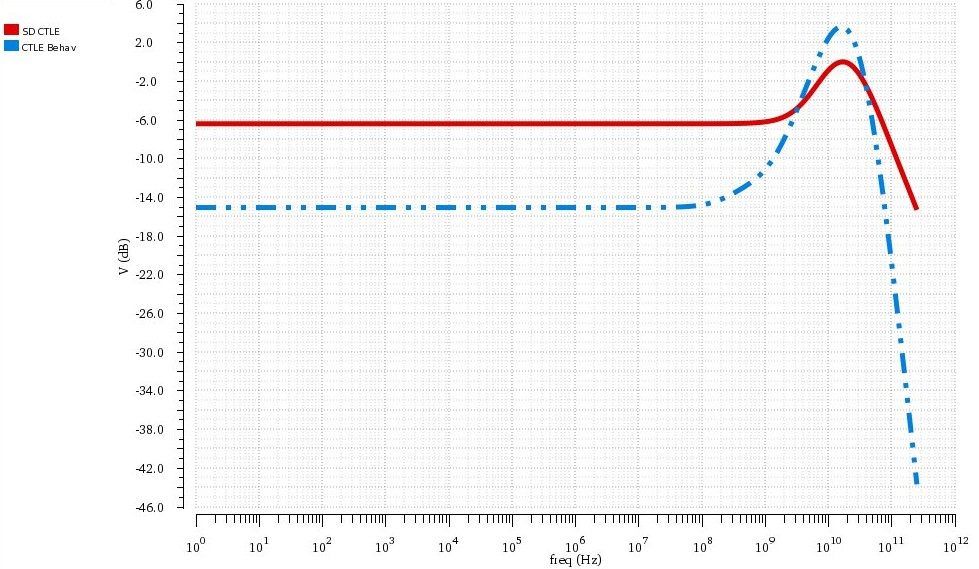
\includegraphics[width=0.85\textwidth]{img/CTLE_img/only_onestage_SD_ctle.jpg}
    \caption{AC response of a single-stage SD CTLE compared with the behavioral model.}
    \label{fig:sd_vs_behav_response}
\end{figure}

\noindent To resolve these performance deficits, the architecture must cascade an additional stage to introduce more poles and zeros, providing the necessary degrees of freedom to tune the response and reach the total required boost. Furthermore, addressing the mid-band attenuation requires a specialized architectural adjustment: by introducing a parallel low-pass path ($G_{m2}$) into the primary stage, the mid-band droop is effectively lifted, creating a smooth, fully compensated equalization profile.

\section*{Proposed Two-Stage Topology}

To overcome the gain and mid-band limitations of the single-stage approach, a two-stage cascaded architecture was developed. As illustrated in Figure~\ref{fig:proposed_topology_block}, the proposed implementation adopts the following cascade:

\begin{figure}[H]
    \centering
    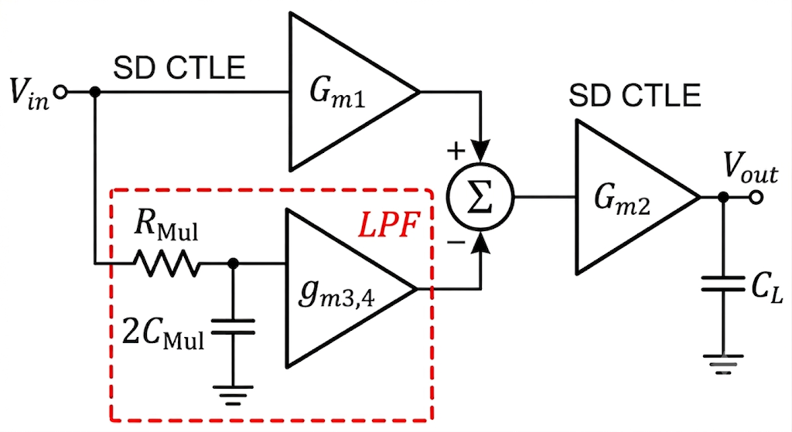
\includegraphics[width=0.7\textwidth]{img/CTLE_img/proposed_topology_block_diagram.png}
    \caption{Block-level diagram of the proposed two-stage CTLE: Stage 1 (Dual-path CTLE) followed by Stage 2 (SD CTLE).}
    \label{fig:proposed_topology_block}
\end{figure}

\begin{enumerate}[noitemsep]
\item \textbf{Stage 1 — Two-Path CTLE:} An SD CTLE augmented with a low-pass $g_m$ branch to compensate for mid-band droop through an additional zero.
\item \textbf{Stage 2 — SD CTLE:} A conventional SD stage that adds a pole/zero pair, increasing high-frequency peaking to reach the \textbf{19 dB} target.
\end{enumerate}

\noindent This cascade provides \textbf{five poles and three zeros}, closely approximating the PCIe 6.0 behavioral reference. The schematic is shown in Figure~\ref{fig:proposed_topology_schematic}.

\begin{figure}[H]
    \centering
    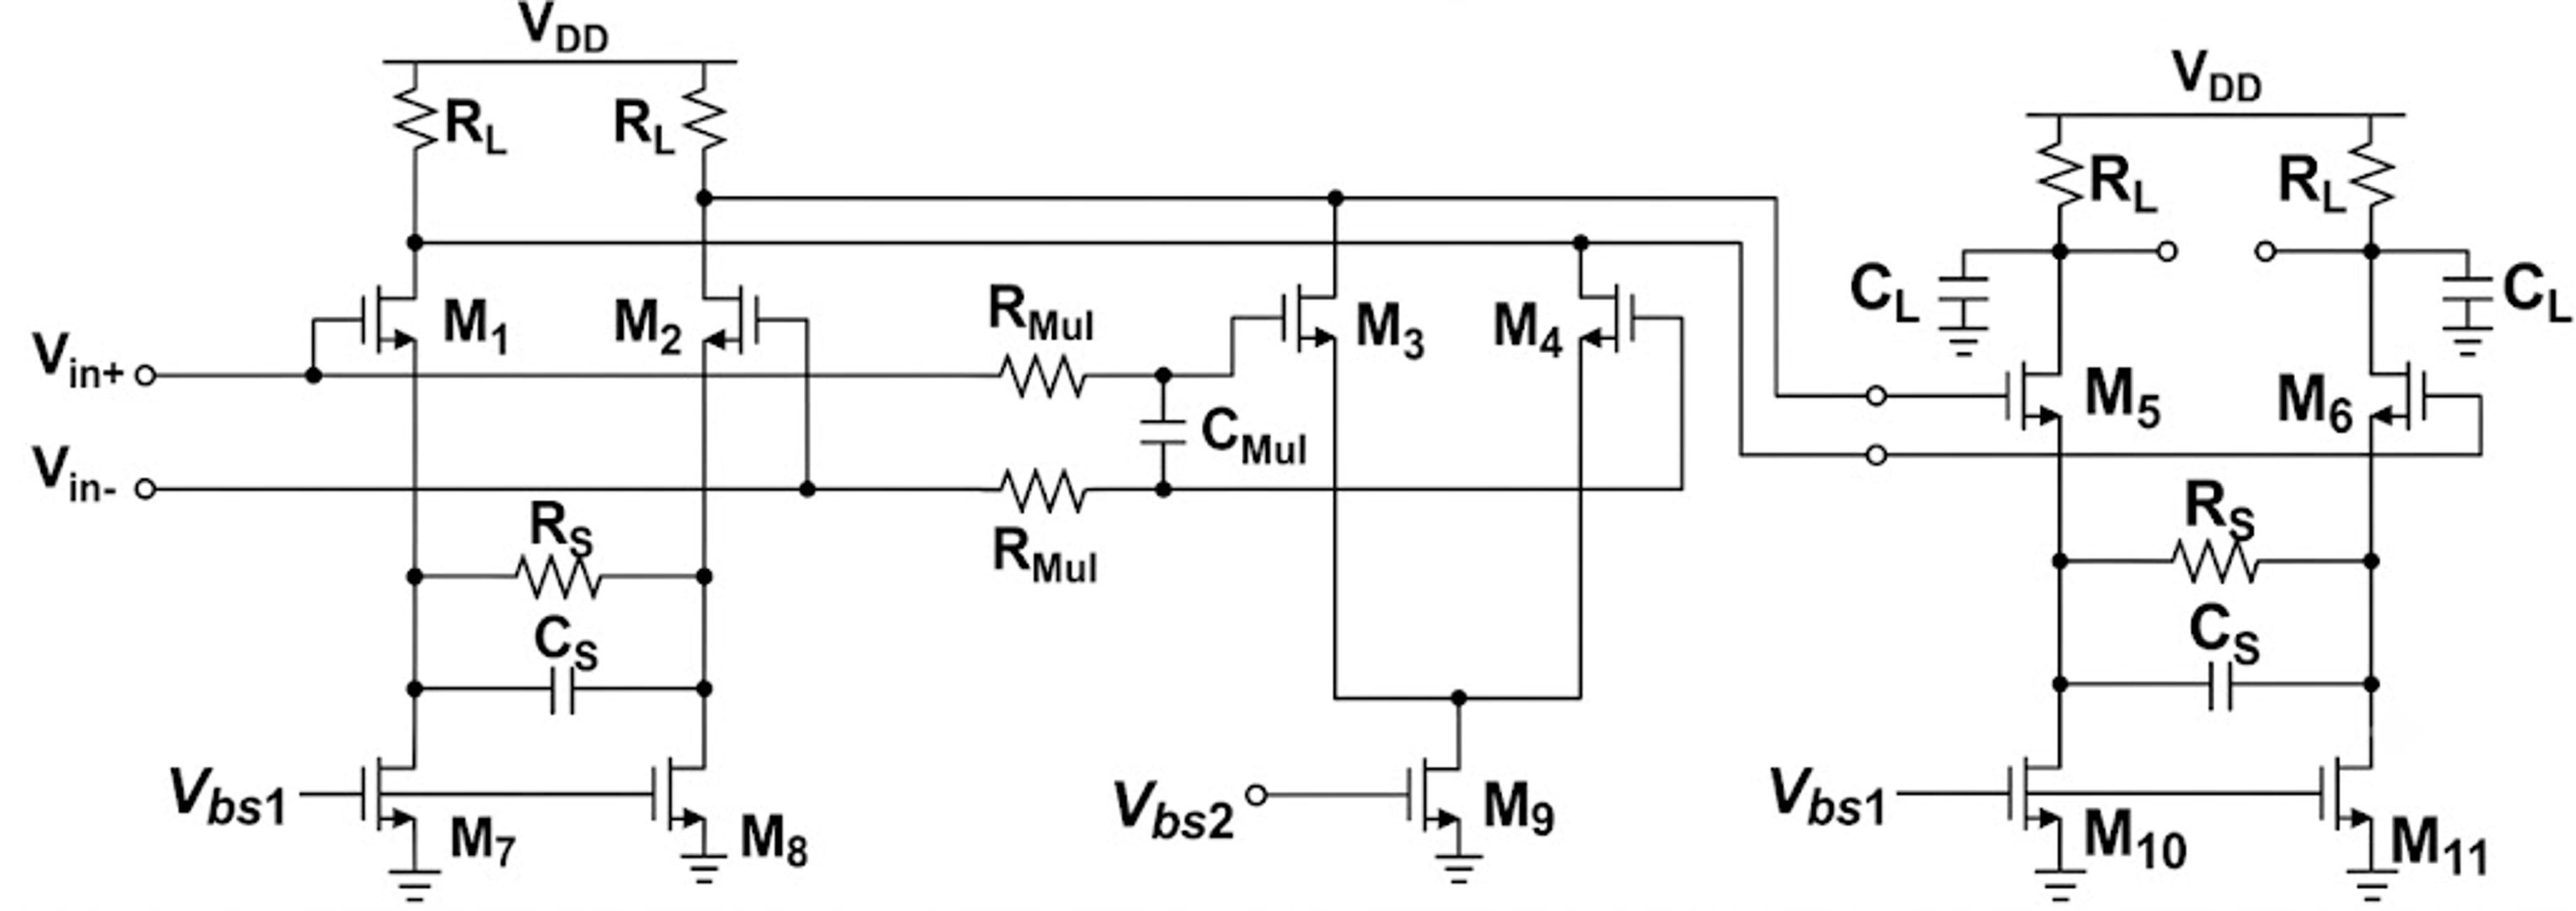
\includegraphics[width=\textwidth]{img/CTLE_img/proposed_topology.png}
    \caption{Transistor-level schematic of the proposed Two-Path + SD CTLE cascaded topology.}
    \label{fig:proposed_topology_schematic}
\end{figure}

\subsection*{Transfer Function}

The overall transfer function of the first stage (Two-path CTLE) is defined by the summation of the main SD path and the secondary low-pass path, given by:

\begin{equation*}
    H_1(s) \simeq -\!\left(\frac{g_{m1,2}}{1+\dfrac{g_{m1,2}R_S}{2}}
    - g_{m3,4}\right)R_L \cdot
    \frac{\left(1+\dfrac{s}{\omega_z}\right)
          \left(1+\dfrac{s}{\omega_{z\_\mathrm{Lpf}}}\right)}
         {\left(1+\dfrac{s}{\omega_{p1}}\right)
          \left(1+\dfrac{s}{\omega_{p2}}\right)
          \left(1+\dfrac{s}{\omega_{p\_\mathrm{Lpf}}}\right)}
    \label{eq:H2}
\end{equation*}

\noindent where the dominant poles and zeros of the main SD path are defined as:
\begin{align*}
    \omega_z       &= \frac{1}{R_S C_S},   \quad
    \omega_{p1}    = \frac{1+g_m R_S/2}{R_S C_S}, \quad
    \omega_{p2}    = \frac{1}{R_L C_L}     \label{eq:poles_sd}
\end{align*}

\noindent and the supplementary mid-band pole and zero introduced by the dual path ($g_{m3,4}$) branch are:
\begin{align*}
    \omega_{z\_\mathrm{Mul}} &= \frac{g_{m1,2}-g_{m3,4}\!\left(1+\frac{g_{m1,2}R_s}{2}\right)}
                                    {2\,g_{m1,2}\,R_{\mathrm{Lpf}}\,C_{\mathrm{Lpf}}},
    \quad
    \omega_{p\_\mathrm{Lpf}} = \frac{1}{2\,R_{\mathrm{Lpf}}\,C_{\mathrm{Lpf}}}
\end{align*}

\noindent The full composite transfer function is given by:

\begin{equation*}
    H_{total}(s) = H_1(s) \cdot H_2(s)
\end{equation*}

\begin{equation*}
    H_{total}(s) = \underbrace{\left[ A_{DC,1} \cdot \frac{(1+\frac{s}{\omega_z})(1+\frac{s}{\omega_{z\_\mathrm{Lpf}}})}{(1+\frac{s}{\omega_{p1}})(1+\frac{s}{\omega_{p2}})(1+\frac{s}{\omega_{p\_\mathrm{Lpf}}})} \right]}_{H_1(s)} \cdot \underbrace{\left[ A_{DC,2} \cdot \frac{(1+\frac{s}{\omega_{z,SD2}})}{(1+\frac{s}{\omega_{p,SD2}})(1+\frac{s}{\omega_{p2,SD2}})} \right]}_{H_2(s)}
\end{equation*}

\begin{equation*}
    A_{DC,total} = -\left[ \left(\frac{g_{m1,2}}{1+\frac{g_{m1,2}R_S}{2}} - g_{m3,4}\right)R_L \right] \cdot \left[ \frac{g_{m,SD2}}{1+\frac{g_{m,SD2}R_{S,SD2}}{2}} R_{L,SD2} \right]
\end{equation*} 
\newline

\noindent Cascading the second SD CTLE stage appends one additional zero ($\omega_z$) and two additional poles ($\omega_{p1}$, $\omega_{p2}$), resulting in the highly tunable five-pole, three-zero composite response required to recover the 64.0 GT/s signal.


\section*{Circuit Design and Analysis}

\subsection{Full Circuit Schematic}

Figure~\ref{fig:full_schematic} displays the complete annotated schematic of the two-stage CTLE, including all back-annotated parasitics. The design utilizes 22\,nm SOI Super-Low VT (SLVT) transistors (\texttt{slvtnfet\_mmw\_5t}) throughout. To model layout interconnects, all signal traces include grey-model back-annotations of $4\,\Omega$ per resistive segment and $5\,\text{fF}$ per capacitive node.

\begin{figure}[H]
    \centering
    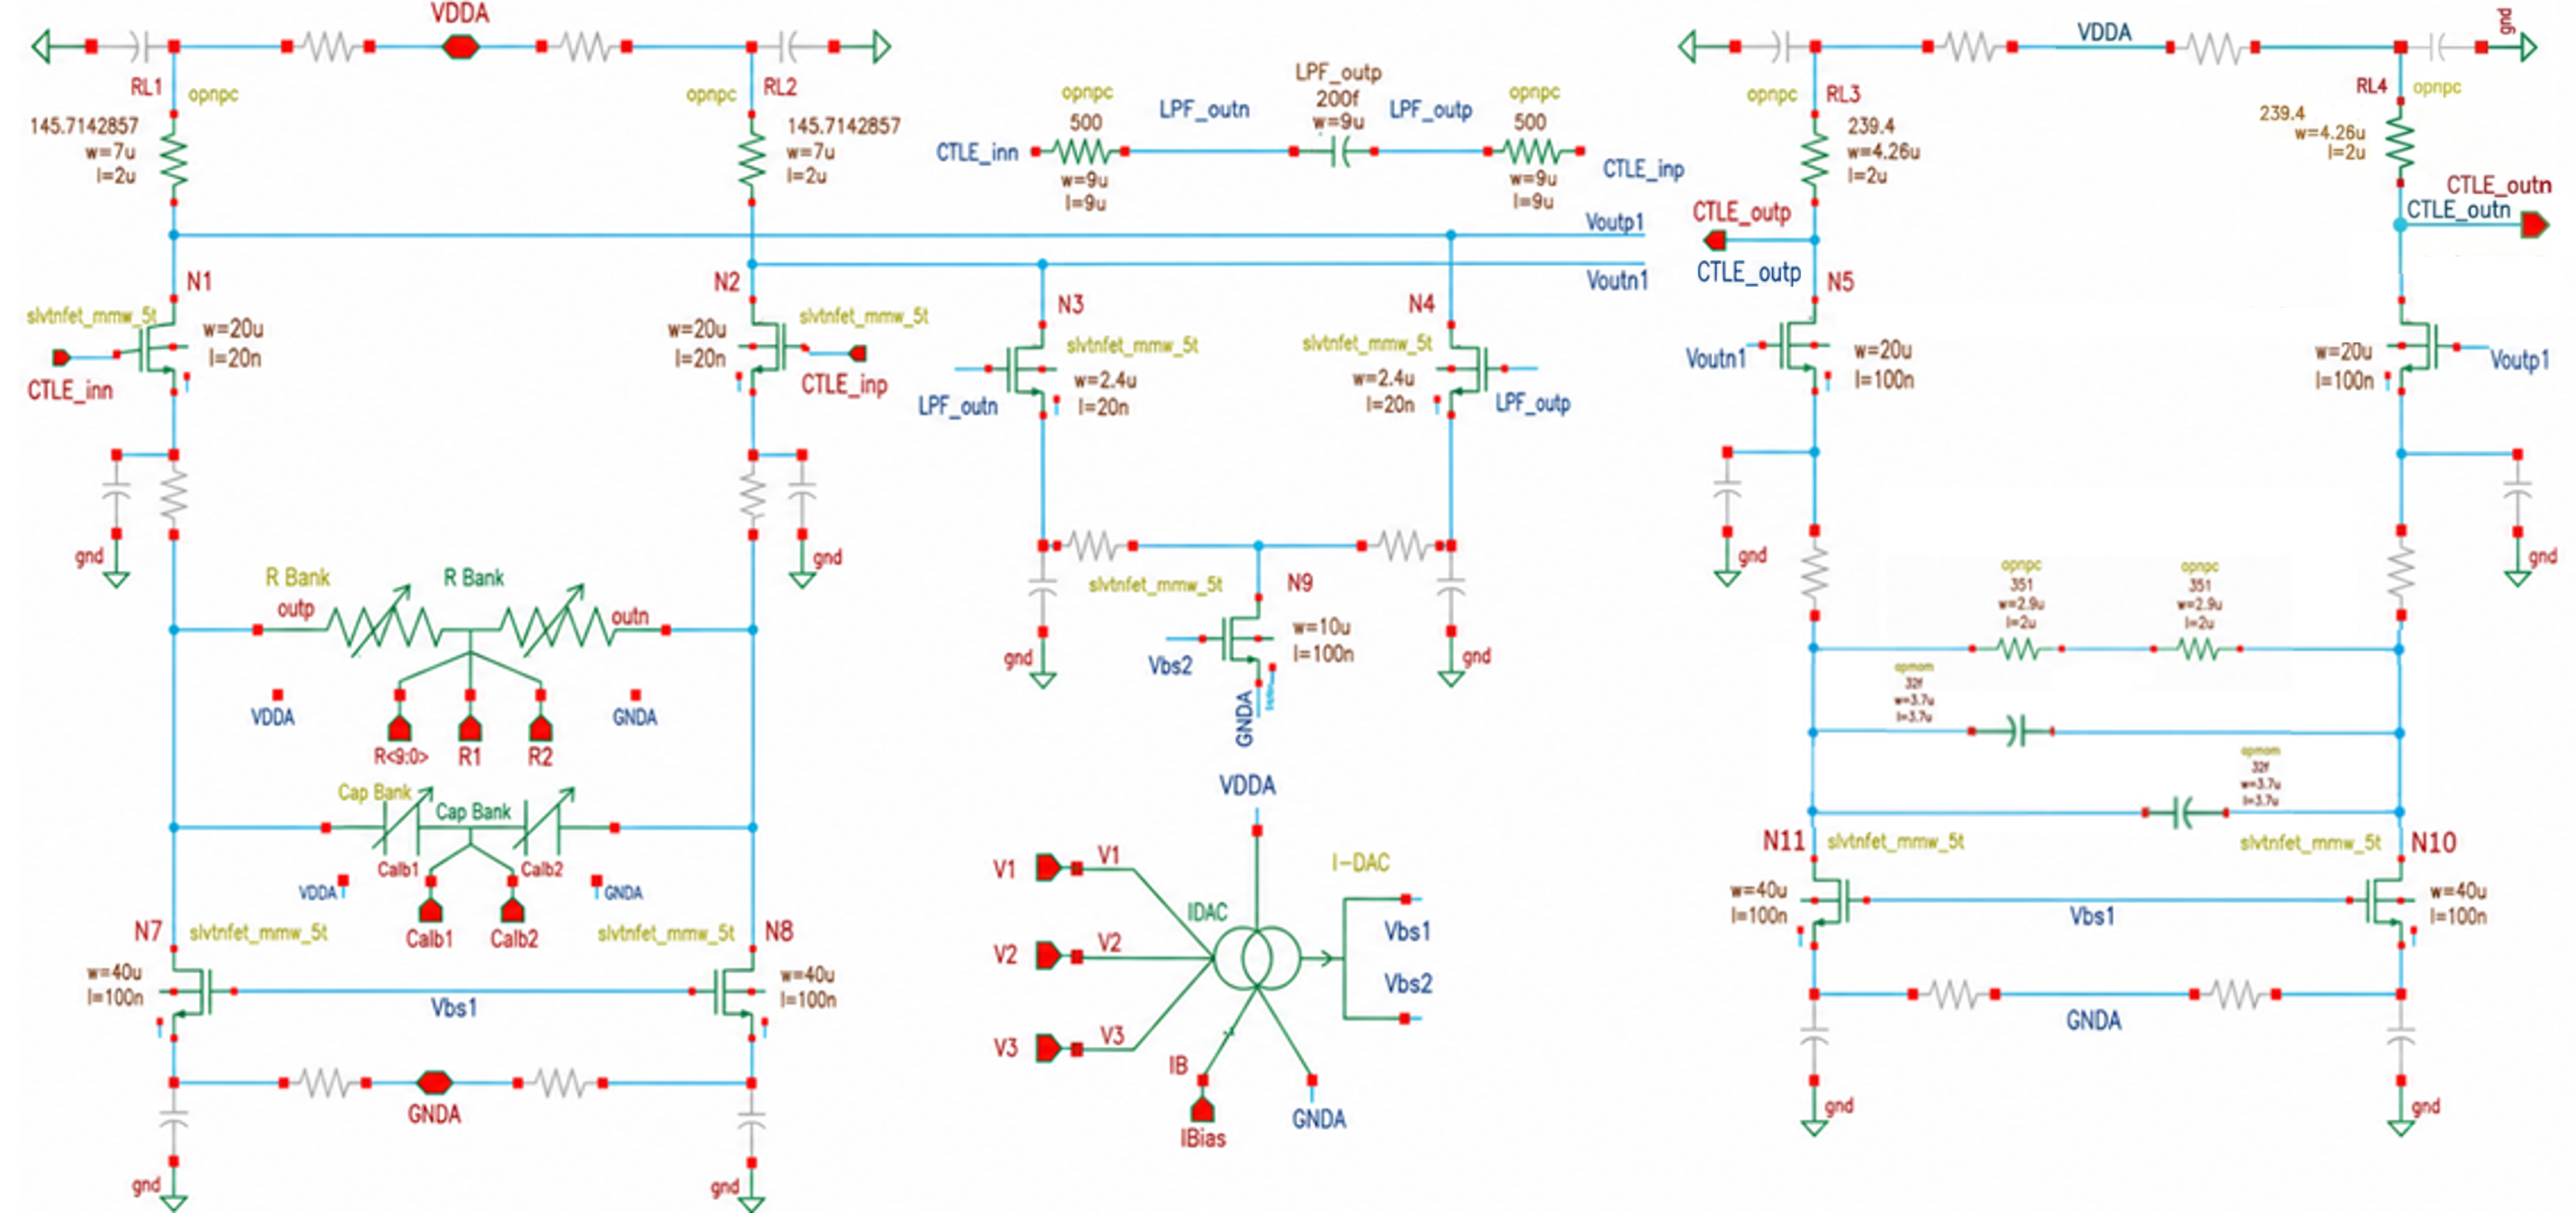
\includegraphics[width=\textwidth]{img/CTLE_img/Circuit_schematic_with_back_annotations.png}
    \caption{Complete annotated schematic of the proposed two-stage CTLE with back-annotated device dimensions and parasitics.}
    \label{fig:full_schematic}
\end{figure}

\subsection*{Stage 1: Dual Path Source-Degenerated CTLE}

The first stage provides the primary tunability for the system. It consists of a high-swing SD CTLE core path augmented with a low-pass multi-path (LPF+$G_{m2}$) branch to flatten mid-band gain.

\subsubsection*{Core Differential Pair and Load ($G_{m1}$)}
The input differential pair ($N_1, N_2$) is sized at $20\,\mu\text{m}/20\,\text{n}\text{m}$, biased by tail current sources ($N_7, N_8$) sized at $40\,\mu\text{m}/100\,\text{n}\text{m}$. The stage utilizes N+ polysilicon load resistors (\texttt{opnpc}) with a value of $145.7\,\Omega$ ($7\,\mu\text{m} \times 2\,\mu\text{m}$ sizing).

\newpage
\subsubsection*{Multi-Path Branch (LPF + Gm cell)}
The secondary low-pass branch ($N_3, N_4$) is sized at $2.4\,\mu\text{m}/20\,\text{n}\text{m}$ with a tail current source ($N_9$) sized at $10\,\mu\text{m}/100\,\text{n}\text{m}$. The branch filter is composed of a $500\,\Omega$ \texttt{opnpc} resistor and an \texttt{apmom} capacitor of $200\,\text{fF}$ ($9\,\mu\text{m} \times 9\,\mu\text{m}$), which sets the mid-band correction frequency. 

\subsubsection*{Tunability}
All DC gain and equalization peaking tunability is centralized in this stage via a programmable resistor bank and capacitive bank, allowing dynamic adjustment of the $R_S-C_S$ degeneration network.

\subsection*{Stage 2: Fixed SD CTLE}

The second stage is a fixed, non-tunable SD CTLE designed for high-frequency boost. To simplify layout, it is architected as a symmetric half-cell, allowing for a mirrored layout implementation.

\subsubsection*{Core Pair and Load}
The input pair ($N_5, N_6$) is sized at $20\,\mu\text{m}/100\,\text{n}\text{m}$ with tail current sources ($40\,\mu\text{m}/100\,\text{n}\text{m}$). The load resistors are $240\,\Omega$ \texttt{opnpc} ($4.26\,\mu\text{m} \times 2\,\mu\text{m}$).

\subsubsection*{Degeneration Network}
The degeneration network for this stage is fixed and utilizes high-precision \texttt{apmom} and \texttt{opnpc} elements:
\begin{itemize}[noitemsep]
    \item \textbf{Resistors:} Two series identical \texttt{opnpc} resistors, each $351\,\Omega$ ($2.9\,\mu\text{m} \times 2\,\mu\text{m}$).
    \item \textbf{Capacitors:} Two parallel \texttt{apmom} capacitors, each $32\,\text{fF}$ ($3.7\,\mu\text{m} \times 3.7\,\mu\text{m}$).
\end{itemize}

\newpage
\subsection{Thermometer-Coded Resistive Degeneration Bank}
\label{sec:rbank}

The DC gain of the CTLE is controlled by varying the effective source-degeneration resistance $R_S$ using a thermometer-coded resistive bank. As shown in Figure~\ref{fig:rbank}, this bank utilizes a set of parallel branches, each controlled by the digital thermometer bus $r\langle9:0\rangle$.

\begin{figure}[H]
    \centering
    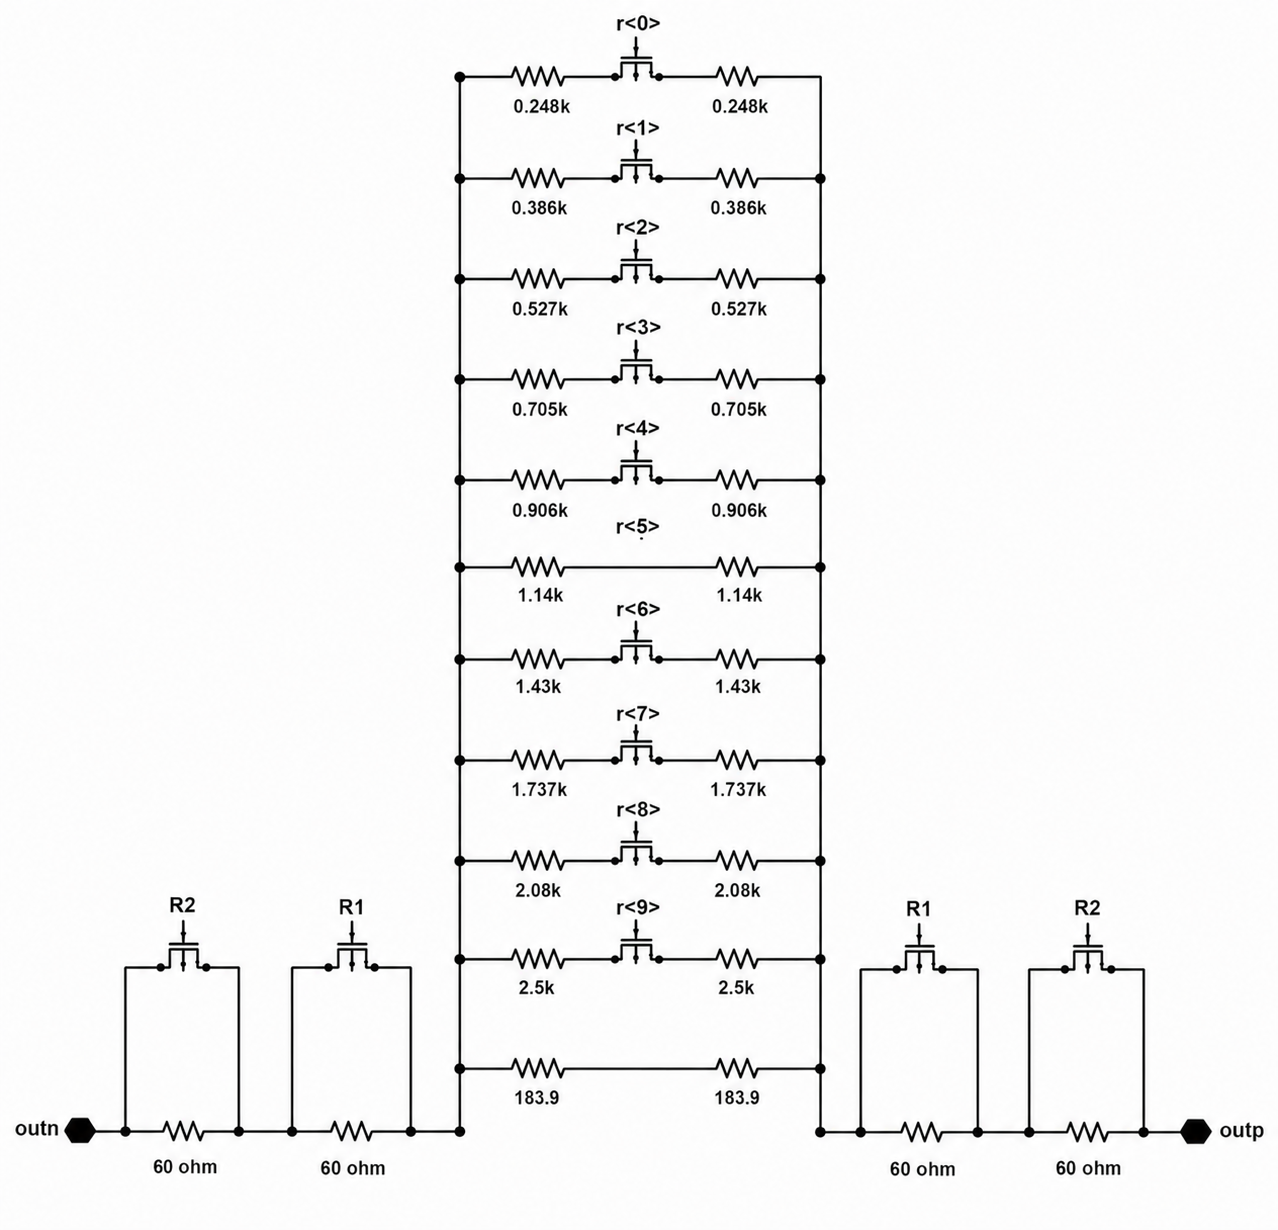
\includegraphics[width=0.8\textwidth]{img/CTLE_img/Resistor_bank_schematic.png}
    \caption{Schematic of the thermometer-coded degeneration resistive bank used for DC gain control and PVT compensation.}
    \label{fig:rbank}
\end{figure}

\subsection*{Gain Control Logic}
The bank operates by selectively activating parallel branches to adjust the total degeneration resistance $R_S$, which in turn controls the DC gain and peaking according to:
\begin{equation*}
    A_{\mathrm{DC}} \approx \frac{g_{m1,2}\,R_L}{1+g_{m1,2}R_S/2},
    \qquad
    \mathrm{Boost} = 1 + \frac{g_m R_S}{2}
\end{equation*}

\noindent The bank includes PVT compensation via control signals $R_1$ and $R_2$, which are gate signals for switches placed in parallel with specific degeneration resistors. When a gate signal (e.g., $R_1$ or $R_2$) is asserted (HIGH), the respective switch is turned ON, shorting the resistor in parallel with it.
\newpage Each switch is designed with an on-resistance ($R_{on}$) of approximately $10\,\Omega$, which is accounted for in the effective resistance when a branch is active.

The gain control follows a structured activation sequence:
\begin{itemize}
    \item \textbf{-15 dB (Minimum Gain/ Max Peaking):} All parallel branches controlled by $r\langle9:0\rangle$ are disabled. The degeneration is provided solely by the "always-active" branch, which contains two series resistors without an associated switch.
    \item \textbf{-14 dB:} Only $r\langle9\rangle$ is activated, placing its branch in parallel with the always-active branch.
    \item \textbf{-13 dB:} $r\langle9\rangle$ and $r\langle8\rangle$ are activated in parallel.
    \item \textbf{-12 dB:} $r\langle9\rangle$, $r\langle8\rangle$, and $r\langle7\rangle$ are activated.
    \item[] \hfil$\vdots$\hfil
    \item \textbf{-5 dB (Maximum Gain/ Min Peaking):} All parallel branches are active, providing minimum degeneration.
\end{itemize}
This thermometer-coded approach ensures monotonic gain steps and prevents transient glitches during state transitions.

\subsection*{PVT Corner Compensation}
To maintain consistent performance across PVT corners, two fixed resistors, $R_1$ and $R_2$, are incorporated to compensate for resistance degradation:
\begin{itemize}
    \item \textbf{$R_2$:} This resistor is permanently included in all Fast-Fast (FF) corners to prevent excessive gain due to increased transistor mobility and lower effective resistance values.
    \item \textbf{$R_1$:} This resistor is selectively engaged only in the FF125$^{\circ}$C ($-5\% V_{DD}$) corner to provide additional degeneration, counteracting the gain increase and maintaining the target equalization profile.
\end{itemize}


\newpage
\subsection{Capacitive Degeneration Bank}
\label{sec:capbank}

The capacitive degeneration bank tunes the zero frequency ($\omega_z = 1/R_S C_S$) to stabilize the CTLE peaking profile across process, voltage, and temperature (PVT) variations. As shown in Figure~\ref{fig:cap_bank}, the bank uses calibration signals \texttt{calib0} and \texttt{calib1} to adjust the total effective degeneration capacitance ($C_S$).

\begin{figure}[H]
    \centering
    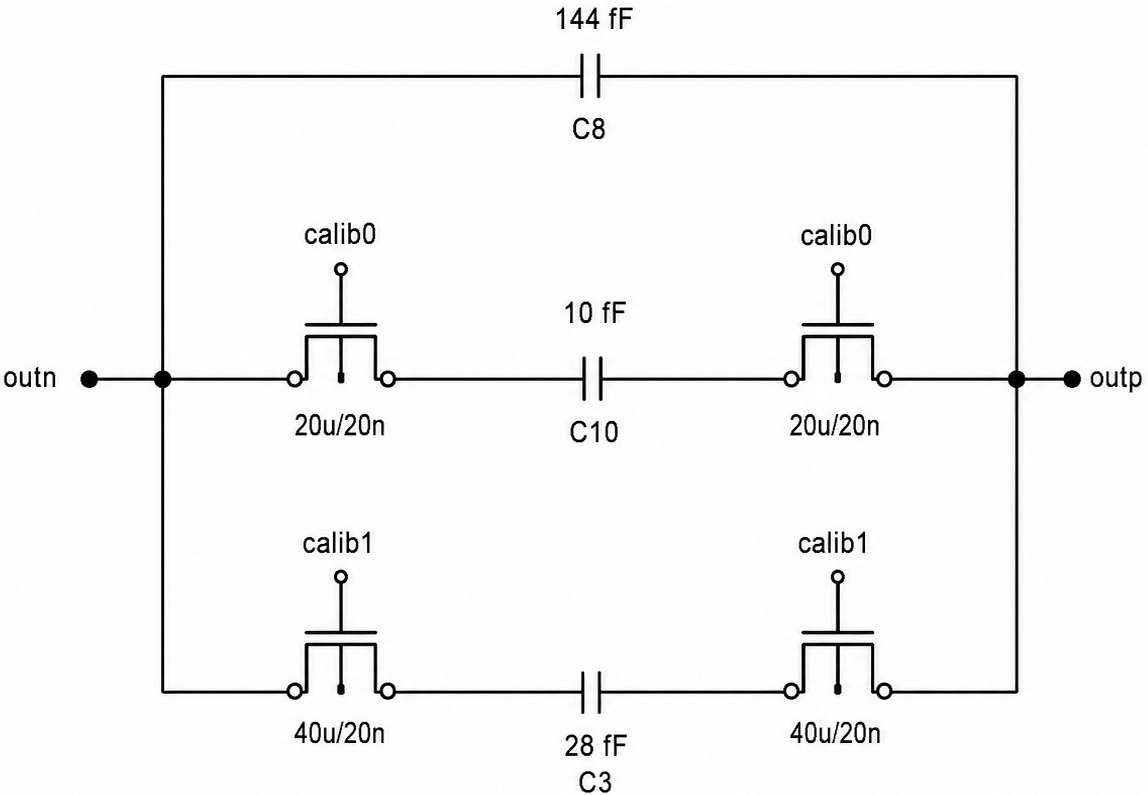
\includegraphics[width=0.7\textwidth]{img/CTLE_img/cap_bank.png}
    \caption{Capacitive degeneration bank schematic using \texttt{calib0} and \texttt{calib1} for PVT-dependent peaking adjustment.}
    \label{fig:cap_bank}
\end{figure}

\subsection*{Principle of Operation}
The network defaults to a base capacitance when \texttt{calib0} and \texttt{calib1} are inactive. Asserting these signals closes the respective switches, adding capacitors in parallel to $C_S$. This tunability compensates for process-induced shifts in transconductance ($g_m$):

\begin{itemize}
    \item \textbf{Typical-Typical (TT) Corner (\texttt{calib0}=VDD, \texttt{calib1}=0):} Sets the nominal capacitive load.
    \item \textbf{Fast-Fast (FF) Corner (\texttt{calib0}=VDD, \texttt{calib1}=VDD):} Higher mobility increases intrinsic peaking. Adding capacitance shifts $\omega_z$ lower, dampening excessive high-frequency gain to restore the target profile.
    \item \textbf{Slow-Slow (SS) Corner (\texttt{calib0}=0, \texttt{calib1}=0):} Lower mobility degrades peaking. Minimizing $C_S$ shifts $\omega_z$ higher, reducing high-frequency degeneration to recover the necessary gain boost.
\end{itemize}

By dynamically adjusting $C_S$, the bank centers the CTLE peaking at the Nyquist frequency, decoupling the equalization magnitude from process-dependent $g_m$ variations.

\subsection{Biasing Network}
\label{sec:bias}

The biasing network is responsible for generating the stable gate bias voltages ($V_{\mathrm{bs1}}$ and $V_{\mathrm{bs2}}$) required by the CTLE tail current sources. To ensure robust equalization performance across all PVT corners, the network utilizes a digitally controlled, custom-weighted current DAC (I-DAC) architecture that regulates the nominal $1.05\,\text{mA}$ reference current.

Figure~\ref{fig:bias_schematic} illustrates the complete top-level schematic of the I-DAC, highlighting the current-steering network divided into parallel weighted branches to provide high-resolution dynamic range.

\begin{figure}[H]
    \centering
    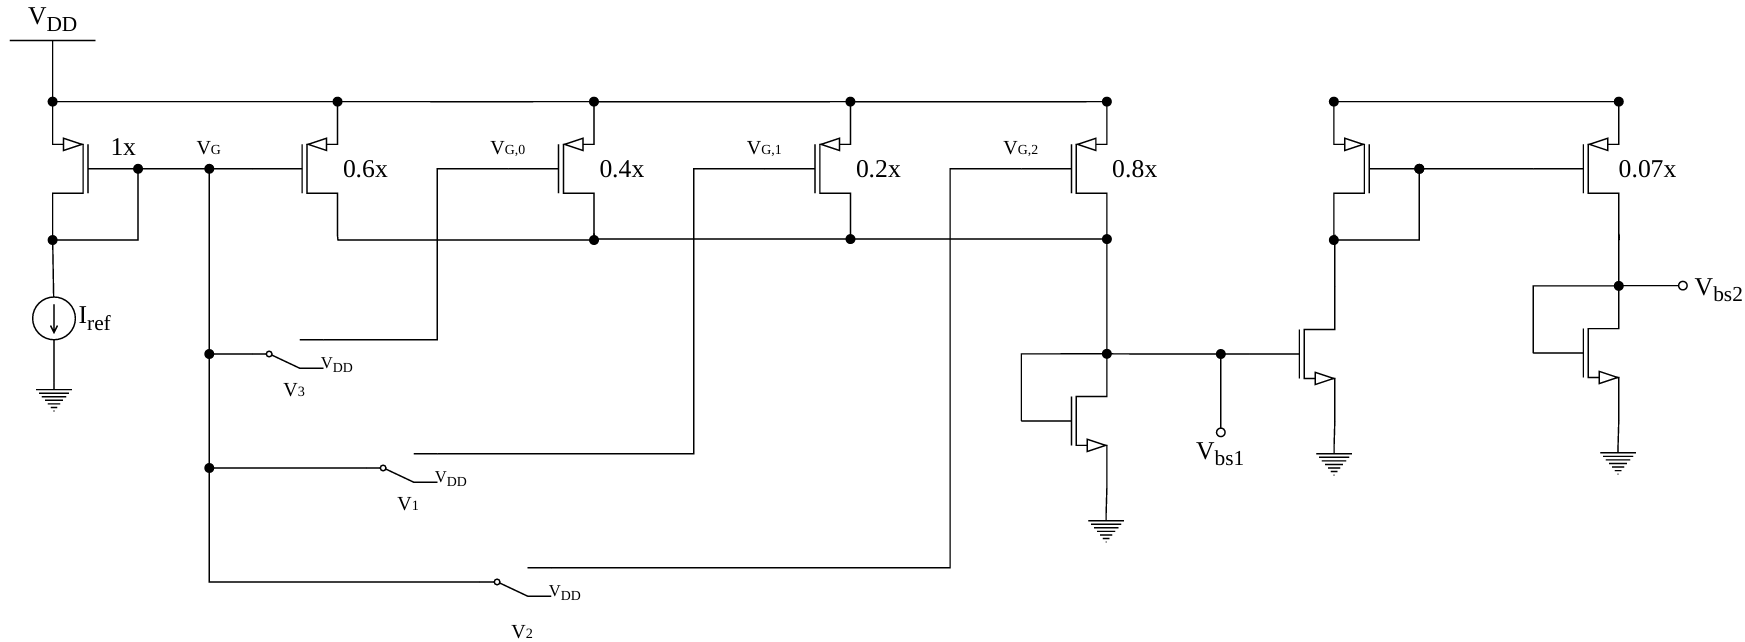
\includegraphics[width=0.95\textwidth]{img/CTLE_img/bias_schematic.png}
    \caption{Biasing network schematic featuring the custom-weighted I-DAC architecture. The network utilizes parallel branches with specific fractional weights of the reference current.}
    \label{fig:bias_schematic}
\end{figure}

\subsection*{Principle of Operation and Custom Weighting}
The I-DAC provides the necessary dynamic range to actively counteract PVT-induced variations in the equalizer's transconductance ($g_m$). The total reference current is distributed across four distinct, precisely weighted branches:
\begin{itemize}[noitemsep]
    \item \textbf{Base Branch (Always-On):} A fixed branch provides a minimum of $60\%$ of the reference current, ensuring the CTLE maintains a stable baseline operation under all conditions (e.g., preventing complete shut-off during extreme Slow-Slow corners).
    \item \textbf{V3 Control Branch ($40\%$):} Controlled by digital signal V3, supplying $40\%$ of the nominal current.
    \item \textbf{V1 Control Branch ($20\%$):} Controlled by digital signal V1, supplying $20\%$ of the nominal current.
    \item \textbf{V2 Control Branch ($80\%$):} Controlled by digital signal V2, supplying $80\%$ of the nominal current.
\end{itemize}

By asserting the appropriate combination of the V1, V2, and V3 control bits, the total bias current can be scaled from a minimum of $60\%$ up to a maximum of $200\%$ of the nominal value. This wide programmable range is heavily utilized in Fast-Fast (FF) corners to scale up the current and compensate for mobility-driven performance shifts, while allowing selective deactivation in Slow-Slow (SS) corners to prevent the bias current from exceeding target margins and causing excessive gain.

\subsection*{2-Way Branch Switching Mechanism}
To cleanly activate and deactivate the dynamically weighted branches without disturbing the primary reference diode, a custom 2-way switch topology is implemented, as detailed in Figure~\ref{fig:bias_switch}.

\begin{figure}[H]
    \centering
    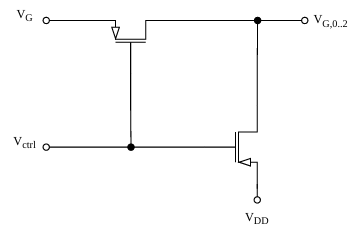
\includegraphics[width=0.50\textwidth]{img/CTLE_img/2way_switch.png}
    \caption{Schematic of the 2-way switch topology used to activate or deactivate the individual weighted PMOS current mirror branches.}
    \label{fig:bias_switch}
\end{figure}

When a specific branch is disabled by its digital control signal ($V_{\text{ctrl}}$), the 2-way switch actively pulls the gate voltage of that branch's PMOS mirror device directly to $V_{\mathrm{DD}}$. This entirely shuts off the transistor, eliminating sub-threshold leakage. Conversely, when enabled, the switch seamlessly connects the gate to the primary diode-connected control voltage ($V_G$), allowing the branch to accurately mirror its designated fractional current.

\subsection*{Multi-Stage Mirroring}
The network employs five primary PMOS mirrors ($30\,\mu\text{m}/100\,\text{n}\text{m}$) and utilizes minimum-sized devices ($2.4\,\mu\text{m}/20\,\text{n}\text{m}$) for the 2-way control switches to minimize parasitic gate capacitance. To support the low-pass filter (LPF) branch's substantially lower current requirement of $70\,\mu\text{A}$, a secondary local NMOS mirror is implemented. This secondary mirror scales the primary $1.05\,\text{mA}$ reference down to the exact $70\,\mu\text{A}$ required. This hierarchical biasing strategy completely avoids the immense silicon area overhead that would otherwise be required by utilizing excessive high-ratio current multipliers, while effectively stabilizing the CTLE's $g_m$ and peaking frequency across all operating corners.

\newpage
\subsection*{Testbench}
\label{sec:tb}

To validate the two-stage CTLE, a testbench was developed to emulate the severe PCIe 6.0 channel insertion loss. The setup integrates the transistor-level design with bias circuitry, calibration banks, and a thermometer decoder, which generates the control signals for the resistive bank.

\begin{figure}[H]
    \centering
    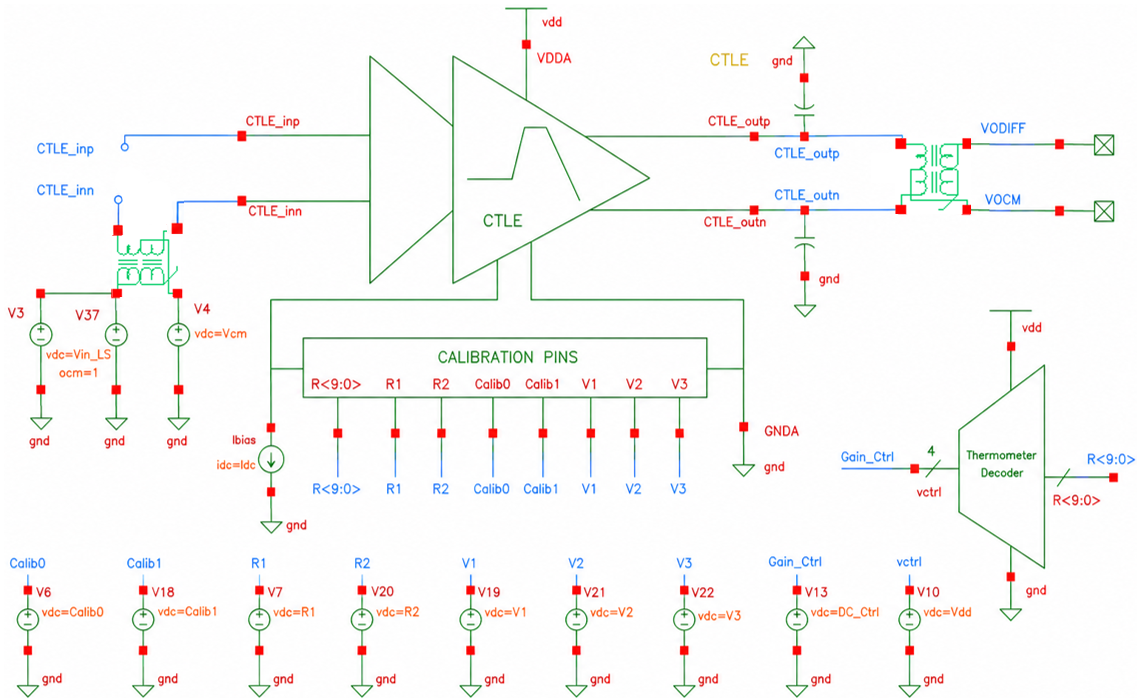
\includegraphics[width=\textwidth]{img/CTLE_img/ctle_test_bench.png}
    \caption{CTLE simulation testbench with thermometer-coded gain control.}
    \label{fig:ctle_testbench}
\end{figure}

\subsection*{Simulation Methodology}
The environment performs the following analyses:
\begin{itemize}[noitemsep]
    \item \textbf{AC Analysis:} Measures frequency response, peaking magnitude, and mid-band compensation effectiveness.
    \item \textbf{PVT Corner Analysis:} Evaluates gain and calibration robustness across FF, SS, and TT corners to ensure stable equalization under extreme conditions.
    \item \textbf{Transient Analysis:} Assesses 64.0\,GT/s signal integrity. The input includes the PCIe 6.0 channel and matching network to confirm the suppression of inter-symbol interference (ISI).
\end{itemize}

\noindent This testbench optimized the design to meet the aggressive \textbf{19 dB} high-frequency boost requirement while maintaining linearity within the 22\,nm SOI process.



\subsection{Simulation Results}
\label{sec:sim_results}

This section details the comprehensive pre-layout simulation results for the proposed two-stage Continuous-Time Linear Equalizer (CTLE). To thoroughly evaluate the design, all simulations were executed within the Cadence Spectre environment utilizing a 22\,nm SOI process technology design kit. Unless otherwise specified, the testing environment assumed a nominal supply voltage of 0.8\,V and an input common-mode voltage ($V_{\mathrm{ICM}}$) of 540\,mV. 

\subsection*{AC Response — Maximum Boost Setting (DC Gain = -15\,dB)}

Figure~\ref{fig:ac_response_2_stages} illustrates the AC frequency response of the equalizer configured at its maximum boost setting, which corresponds to a DC gain of -15\,dB. To provide insight into the distributed equalization strategy, the individual frequency responses of Stage~1 and Stage~2 are plotted independently alongside the cascaded total CTLE response. A behavioral reference model is also superimposed to confirm that the transistor-level implementation accurately tracks the ideal target profile.

\begin{figure}[H]
    \centering
    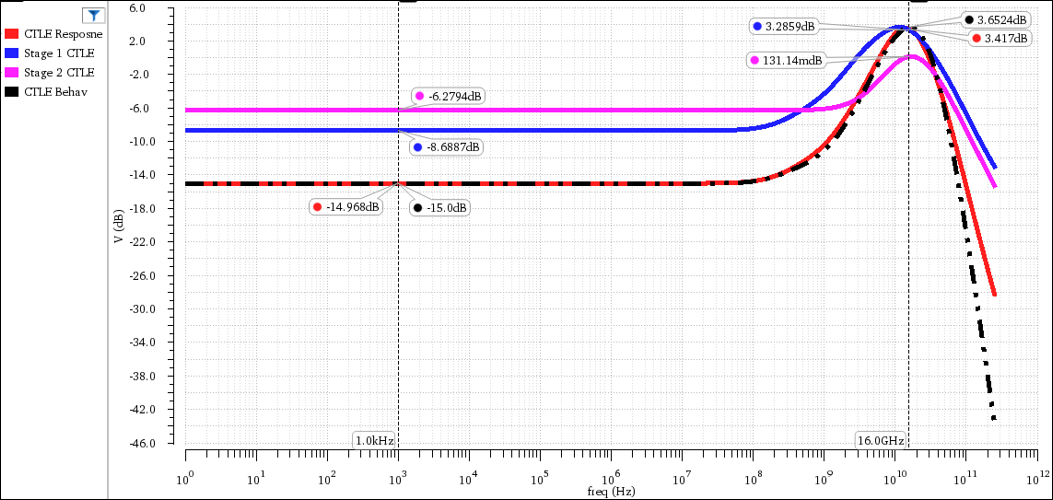
\includegraphics[width=0.90\textwidth]{img/CTLE_img/ac_response_2_stages.png}
    \caption{AC frequency response evaluated at DC gain = -15\,dB ($V_{\mathrm{ICM}} = 540$\,mV).}
    \label{fig:ac_response_2_stages}
\end{figure}

\noindent The key performance metrics extracted from this maximum boost configuration are summarized as follows:
\begin{itemize}[noitemsep]
    \item \textbf{Total DC Gain:} -15.0\,dB
    \item \textbf{Individual Stage DC Gain:} Stage~1 contributes -8.69\,dB; Stage~2 contributes -6.28\,dB.
    \item \textbf{Gain at Nyquist Frequency (16\,GHz):} Peaking achieves between +3.42\,dB and +3.65\,dB.
    \item \textbf{High-Frequency (HF) Boost:} The total effective boost from DC to the Nyquist frequency is approximately 19\,dB.
\end{itemize}

\subsubsection{AC Simulation Across All Gain Settings}

To verify the tunability of the mid-band and low-frequency attenuation, Figure~\ref{fig:ac_response_2_stages_all_settings} presents the cascaded CTLE frequency response across all eleven discrete gain settings. The DC gain is swept from its maximum value of -5\,dB down to its minimum value of -15\,dB, with the measured DC gain annotated directly on each corresponding curve.

\begin{figure}[H]
    \centering
    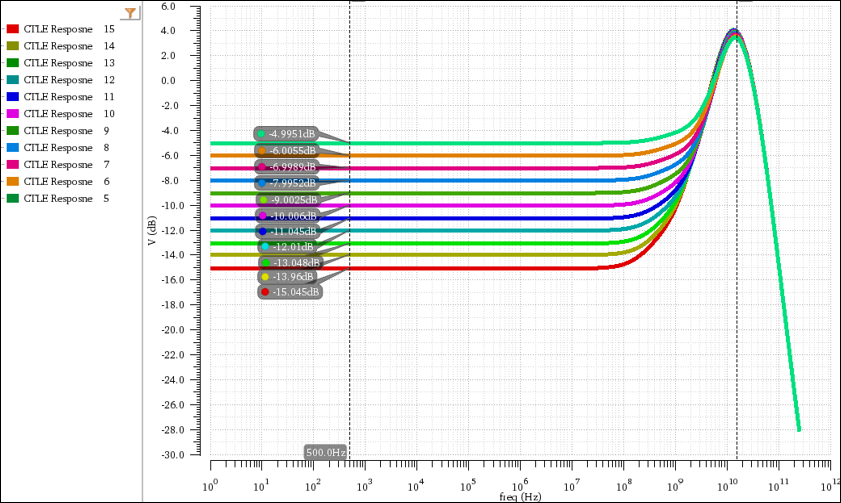
\includegraphics[width=0.90\textwidth]{img/CTLE_img/ac_response_2_stages_all_settings.png}
    \caption{Family of AC frequency response curves representing all eleven DC gain control settings.}
    \label{fig:ac_response_2_stages_all_settings}
\end{figure}

\noindent The operation of the thermometer-coded resistive degeneration bank ensures that the gain steps are highly uniform. The design achieves monotonic steps of approximately 1\,dB throughout the entire control range. The precise measured DC gain for each digital control word is documented in Table~\ref{tab:dc_gain_values}.

\begin{table}[H]
    \centering
    \caption{Measured low-frequency DC gain values for all eleven programmable gain control settings.}
    \label{tab:dc_gain_values}
    \begin{tabular}{cc|cc}
        \toprule
        \textbf{DC\_Ctrl} & \textbf{DC Gain (dB)} & \textbf{DC\_Ctrl} & \textbf{DC Gain (dB)} \\
        \midrule
        5  & $-4.995$  & 11 & $-11.045$ \\
        6  & $-6.006$  & 12 & $-12.010$ \\
        7  & $-6.999$  & 13 & $-13.048$ \\
        8  & $-7.995$  & 14 & $-13.960$ \\
        9  & $-9.003$  & 15 & $-15.045$ \\
        10 & $-10.006$ &    &           \\
        \bottomrule
    \end{tabular}
\end{table}

\subsubsection*{Input and Output Swing — Linearity Analysis}
Maintaining signal linearity is critical to prevent the equalizer from introducing harmonic distortion into the data stream. Linearity was analyzed by sweeping the differential input amplitude and measuring the fundamental harmonic of the output signal.

\subsubsection*{High Boost Setting (DC Gain = -15\,dB)}
Figure~\ref{fig:ctle_gain_linearity_gain_15dB_1db_compression} evaluates the CTLE gain linearity at the highest boost setting, using a 1\,kHz test tone with a baseline differential input of 0.5\,V$_{\text{pp,diff}}$. The corresponding time-domain waveforms are shown in Figure~\ref{fig:ctle_gain_linearity_gain_15dB_sinwave}.

\begin{figure}[H]
    \centering
    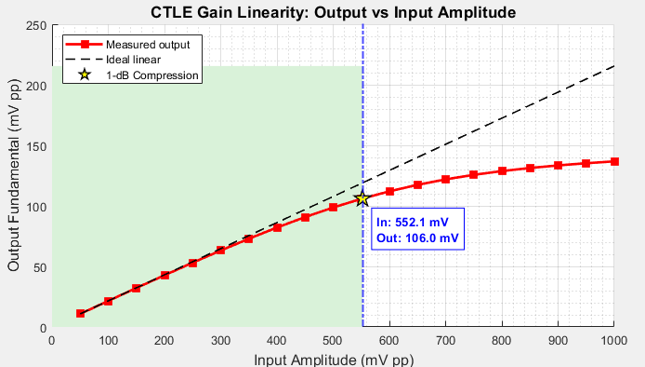
\includegraphics[width=0.8\textwidth]{img/CTLE_img/ctle_gain_linearity_gain_15dB_1db_compression.png}
    \caption{CTLE gain linearity characteristics (output fundamental amplitude versus input amplitude) configured at DC gain = -15\,dB.}
    \label{fig:ctle_gain_linearity_gain_15dB_1db_compression}
\end{figure}

\begin{figure}[H]
    \centering
    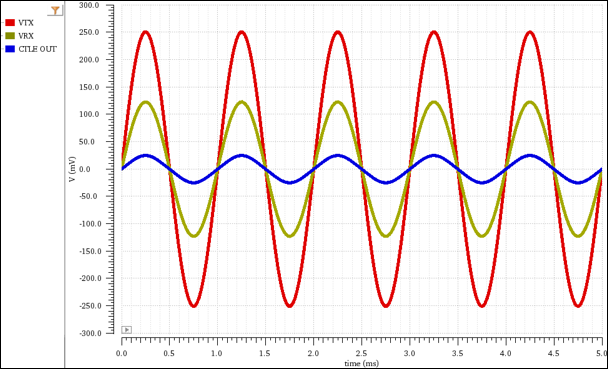
\includegraphics[width=0.8\textwidth]{img/CTLE_img/ctle_gain_linearity_gain_15dB_sinwave.png}
    \caption{Time-domain waveforms at DC gain = -15\,dB, illustrating the input and output voltage swings.}
    \label{fig:ctle_gain_linearity_gain_15dB_sinwave}
\end{figure}

The extracted linearity parameters at the maximum boost configuration are:
\begin{itemize}[noitemsep, topsep=0pt]
    \item \textbf{1-dB Compression Point:} Reached at an input of 552.1\,mV, corresponding to an output of 106.0\,mV.
    \item \textbf{Linear Input Range:} The circuit maintains a linear response up to approximately 1.1\,V$_{\text{pp,diff}}$.
    \item \textbf{Output Swing:} The available linear output swing is approximately 210\,mV$_{\text{pp,diff}}$.
\end{itemize}

\subsubsection*{Low Boost Setting (DC Gain = -5\,dB)}

Figure~\ref{fig:ctle_gain_linearity_gain_5dB_1db_compression} repeats this linearity characterization, configuring the equalizer to its minimum boost setting (maximum DC gain). The corresponding time-domain waveforms are shown in Figure~\ref{fig:ctle_gain_linearity_gain_5dB_sinwave}.

\begin{figure}[H]
    \centering
    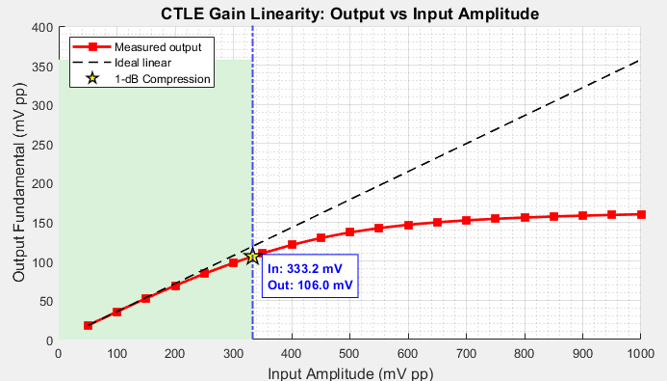
\includegraphics[width=0.75\textwidth]{img/CTLE_img/ctle_gain_linearity_gain_5dB_1db_compression.png}
    \caption{CTLE gain linearity characteristics evaluated at DC gain = -5\,dB.}
    \label{fig:ctle_gain_linearity_gain_5dB_1db_compression}
\end{figure}

\begin{figure}[H]
    \centering
    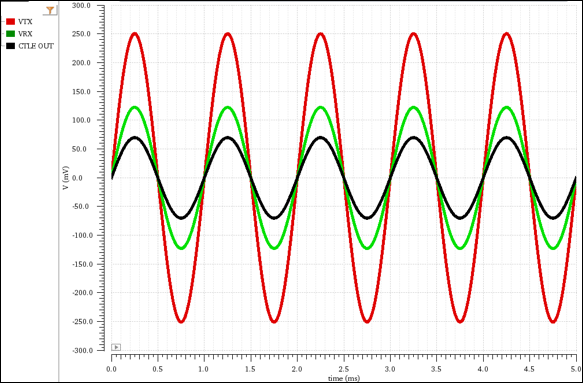
\includegraphics[width=0.75\textwidth]{img/CTLE_img/ctle_gain_linearity_gain_5dB_sinwave.png}
    \caption{Time-domain waveforms at DC gain = -5\,dB, illustrating the input and output voltage swings.}
    \label{fig:ctle_gain_linearity_gain_5dB_sinwave}
\end{figure}

The extracted linearity parameters at the minimum boost configuration are:
\begin{itemize}[noitemsep]
    \item \textbf{1-dB Compression Point:} Reached earlier due to higher DC gain, occurring at an input of 333.2\,mV with an output of 106.0\,mV.
    \item \textbf{Linear Input Range:} The linear input boundary shifts to approximately 660\,mV$_{\text{pp,diff}}$.
    \item \textbf{Output Swing:} The available linear output swing remains steady at approximately 210\,mV$_{\text{pp,diff}}$.
\end{itemize}

\subsubsection{Noise Analysis}

Figure~\ref{fig:ctle_pnoise} details the simulated broad-spectrum output-referred noise spectral density of the CTLE. At lower frequencies, the noise profile is heavily dominated by flicker ($1/f$) noise. As the frequency increases beyond approximately $1\,\text{MHz}$, the profile transitions into a flat thermal noise floor. 

\begin{figure}[H]
    \centering
    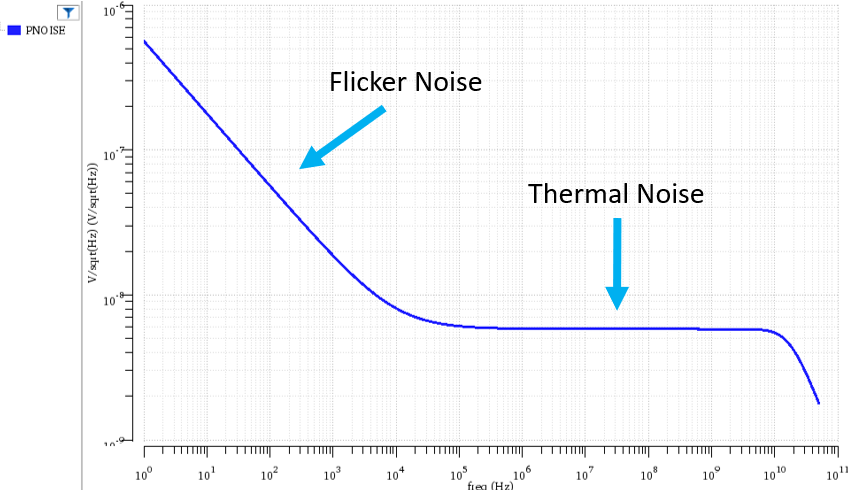
\includegraphics[width=0.90\textwidth]{img/CTLE_img/ctle_pnoise.png}
    \caption{Broadband output-referred noise spectral density profile, highlighting the low-frequency flicker noise region and the transition to the thermal noise floor.}
    \label{fig:ctle_pnoise}
\end{figure}

Figure~\ref{fig:pnoise_peaking} provides a detailed view of the high-frequency spectrum. Importantly, the output noise is actively shaped by the CTLE's frequency response. Because the equalizer applies significant high-frequency voltage gain to compensate for channel insertion loss, it inherently amplifies the thermal noise contribution of the input differential pair. This noise shaping results in a prominent spectral peak in the vicinity of the $16\,\text{GHz}$ Nyquist frequency.



\begin{figure}[H]
    \centering
    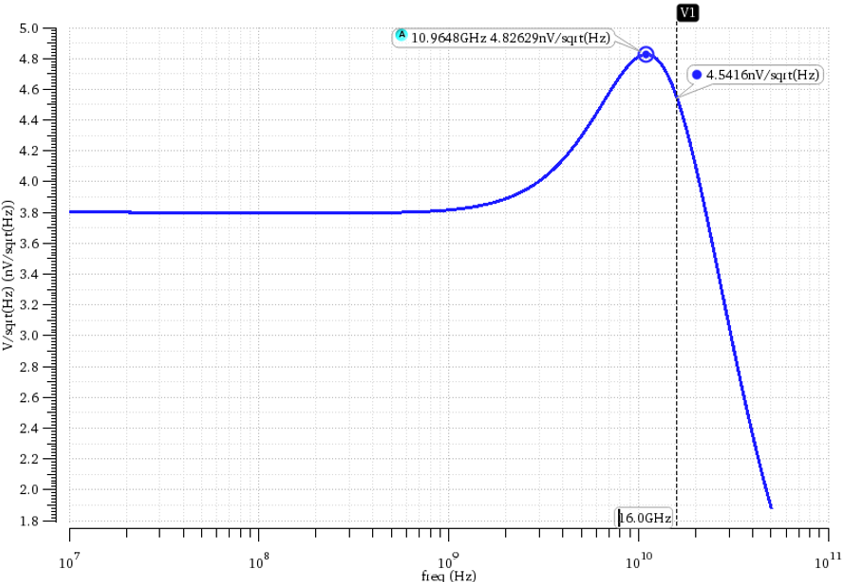
\includegraphics[width=0.90\textwidth]{img/CTLE_img/pnoise_peaking.png}
    \caption{High-frequency noise spectral density demonstrating thermal noise \\ shaping by the CTLE gain profile, with a distinct peak near the Nyquist frequency.}
    \label{fig:pnoise_peaking}
\end{figure}

The key quantitative noise measurements are summarized below:
\begin{itemize}[]
    \item \textbf{Total Output-Referred Noise (TT Corner):} The integrated noise across the bandwidth under nominal conditions is $682.1\,\mu\text{V}_{\text{rms}}$.
    \item \textbf{Total Output-Referred Noise (Worst Corner):} The integrated noise increases to a maximum of $767.6\,\mu\text{V}_{\text{rms}}$ under worst-case PVT conditions.
\end{itemize}

\newpage
\subsubsection{Transient Simulation — Single-Bit Response}
To evaluate the time-domain equalization performance, a transient single-bit response (SBR) simulation was executed using a severe $-26$\,dB insertion loss channel model with the equalizer set to a DC gain of $-15$\,dB. The SBR is plotted in Figure~\ref{fig:ctle_sbr} as normalized amplitude against the tap index $k$, where one tap interval corresponds to the Nyquist period ($T_{\mathrm{Nyq}} = 32.5$\,ps). The equalized CTLE output (red) features a sharp main cursor at $k=0$ and rapidly decaying post-cursor ISI, contrasting with the broad, slowly decaying un-equalized channel response (gold).

\begin{figure}[H]
    \centering
    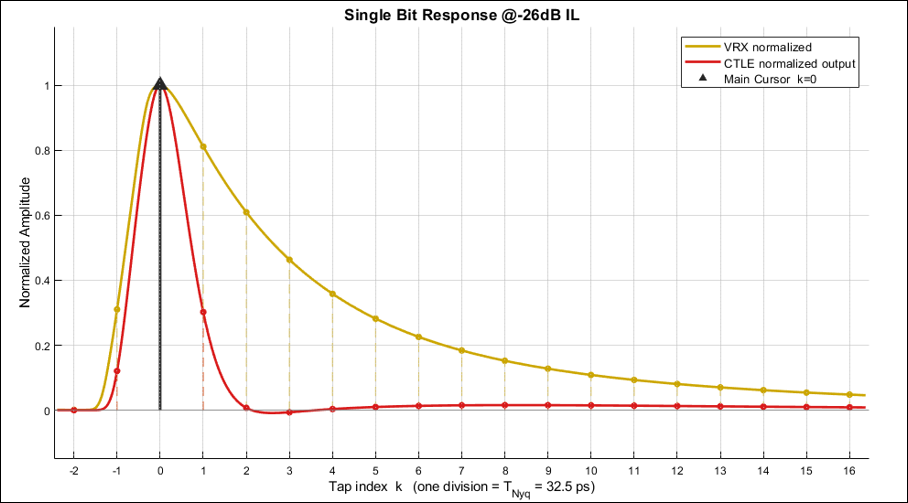
\includegraphics[width=\textwidth]{img/CTLE_img/ctle_sbr.png}
    \caption{Single-bit response (SBR) at $-26$\,dB channel insertion loss, DC gain $= -15$\,dB.}
    \label{fig:ctle_sbr}
\end{figure}

\noindent The results demonstrate that the proposed CTLE significantly compresses the post-cursor ISI tail. While the raw channel impulse response retains substantial energy up to $k = 16$ taps, the equalized output decays to near-zero within just $k = 3$ to $4$ taps, heavily reducing the residual ISI burden on the subsequent Decision Feedback Equalizer (DFE) stage.

\subsubsection{Corner Simulation and PVT Robustness}
AC simulations were conducted across 13 PVT corners, spanning SS/FF process extremes, temperatures of $-40^{\circ}$C and $125^{\circ}$C, and supply voltage variations of $\pm5\%$. At each corner, the 7-bit calibration word (C0, C1, R1, R2, V1, V2, V3) — where C0 and C1 correspond to the capacitive bank control signals Calib0 and Calib1 respectively — is adjusted to maintain the target equalization profile, as documented in Table~\ref{tab:corner_codes}.

\begin{table}[H]
    \centering
    \caption{Digital calibration control codes at each PVT corner (DC gain = $-15$\,dB).}
    \label{tab:corner_codes}
    \resizebox{\textwidth}{!}{%
    \begin{tabular}{lc|lc}
        \toprule
        \textbf{Corner} & \textbf{C0 C1 R1 R2 V1 V2 V3} & \textbf{Corner} & \textbf{C0 C1 R1 R2 V1 V2 V3} \\
        \midrule
        Nominal 27$^{\circ}$C     & 1 0 1 1 0 0 1 & SS $-40^{\circ}$C $-5\%$ & 0 0 1 1 0 0 0 \\
        SS $-40^{\circ}$C         & 0 0 1 1 0 0 0 & FF $-40^{\circ}$C $-5\%$ & 1 1 1 0 1 0 1 \\
        FF $-40^{\circ}$C         & 1 1 1 1 1 0 1 & SS 125$^{\circ}$C $-5\%$ & 1 1 1 1 0 0 1 \\
        SS 125$^{\circ}$C         & 0 0 1 1 0 0 1 & FF 125$^{\circ}$C $-5\%$ & 1 1 0 0 1 1 1 \\
        FF 125$^{\circ}$C         & 1 1 1 0 1 1 1 & SS $-40^{\circ}$C $+5\%$ & 0 0 1 1 0 0 0 \\
        SS 125$^{\circ}$C $+5\%$  & 0 0 1 1 0 0 1 & FF $-40^{\circ}$C $+5\%$ & 1 1 1 1 1 0 1 \\
        FF 125$^{\circ}$C $+5\%$  & 1 1 1 0 1 1 1 & FF 125$^{\circ}$C $+5\%$ & 1 1 1 0 1 1 1 \\
        \bottomrule
    \end{tabular}}
\end{table}

The overlaid frequency responses across all corners are shown in Figure~\ref{fig:ac_response_2_stages_15dB_all_corneres}, with the statistical summary of key metrics provided in Table~\ref{tab:corner_summary}.

\begin{figure}[H]
    \centering
    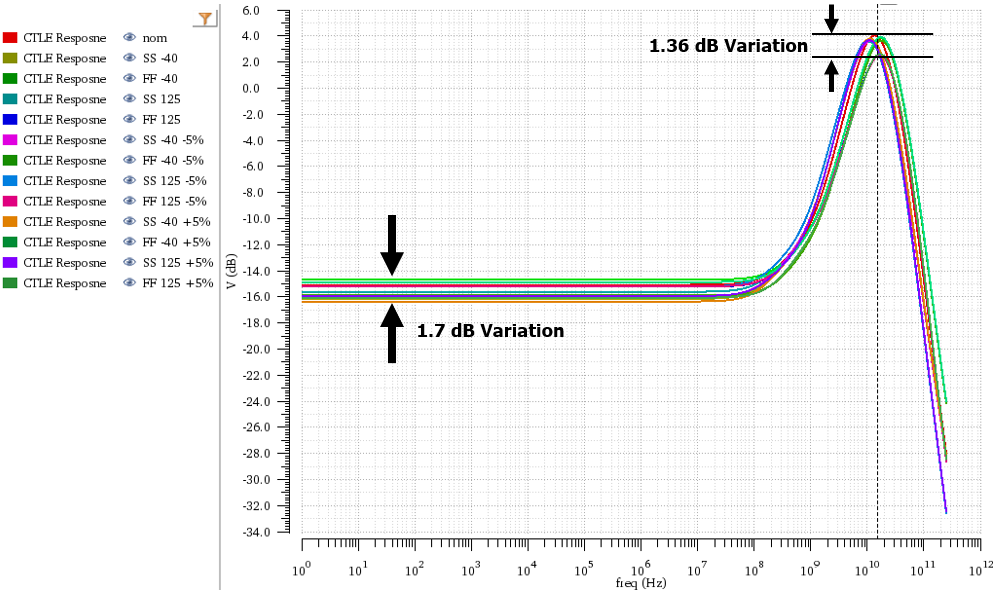
\includegraphics[width=0.90\textwidth]{img/CTLE_img/ac_response_2_stages_15dB_all_corneres.png}
    \caption{Corner simulation frequency responses at DC gain $= -15$\,dB ($V_{\mathrm{ICM}} = 540$\,mV).}
    \label{fig:ac_response_2_stages_15dB_all_corneres}
\end{figure}

\begin{table}[H]
    \centering
    \caption{Statistical summary of corner simulation results at DC gain $= -15$\,dB.}
    \label{tab:corner_summary}
    \begin{tabular}{lrrrl}
        \toprule
        \textbf{Metric}  & \textbf{Min} & \textbf{Max} & \textbf{Mean} & \textbf{Std Dev} \\
        \midrule
        Gain @ $f_{\mathrm{Nyq}}$ (dB)         & 2.27  & 3.87  & 2.97  & 0.49\,dB  \\
        Boost (dB)                              & 8.01  & 20.1  & —  & — \\
        DC Gain (dB)                    & $-16.3$ & $-4.69$  & —  & — \\
        \bottomrule
    \end{tabular}
\end{table}

\noindent All three metrics pass their respective specifications across the complete PVT envelope, with a worst-case DC gain variation of 1.7\,dB and a boost variation of 1.36\,dB.

%% =============================================================
%% CHAPTER 7 – LAYOUT
%% =============================================================
\subsection{Layout Implementation and Post-Layout Verification}
\label{sec:layout_pex}

Transitioning from the schematic to the physical layout requires careful consideration of device matching, signal routing, and parasitic minimization. The layout was meticulously designed to preserve the strict symmetry of the differential signaling path, which is critical for maintaining high common-mode rejection and minimizing even-order harmonic distortion at high frequencies.

\subsubsection{Floorplan and Physical Layout}
As illustrated in the conceptual diagram and the corresponding core layout in Figure~\ref{fig:layout_floorplan}, the components are arranged systematically to preserve differential symmetry. 

\begin{figure}[H]
    \centering
    \begin{minipage}{0.48\textwidth}
        \centering
        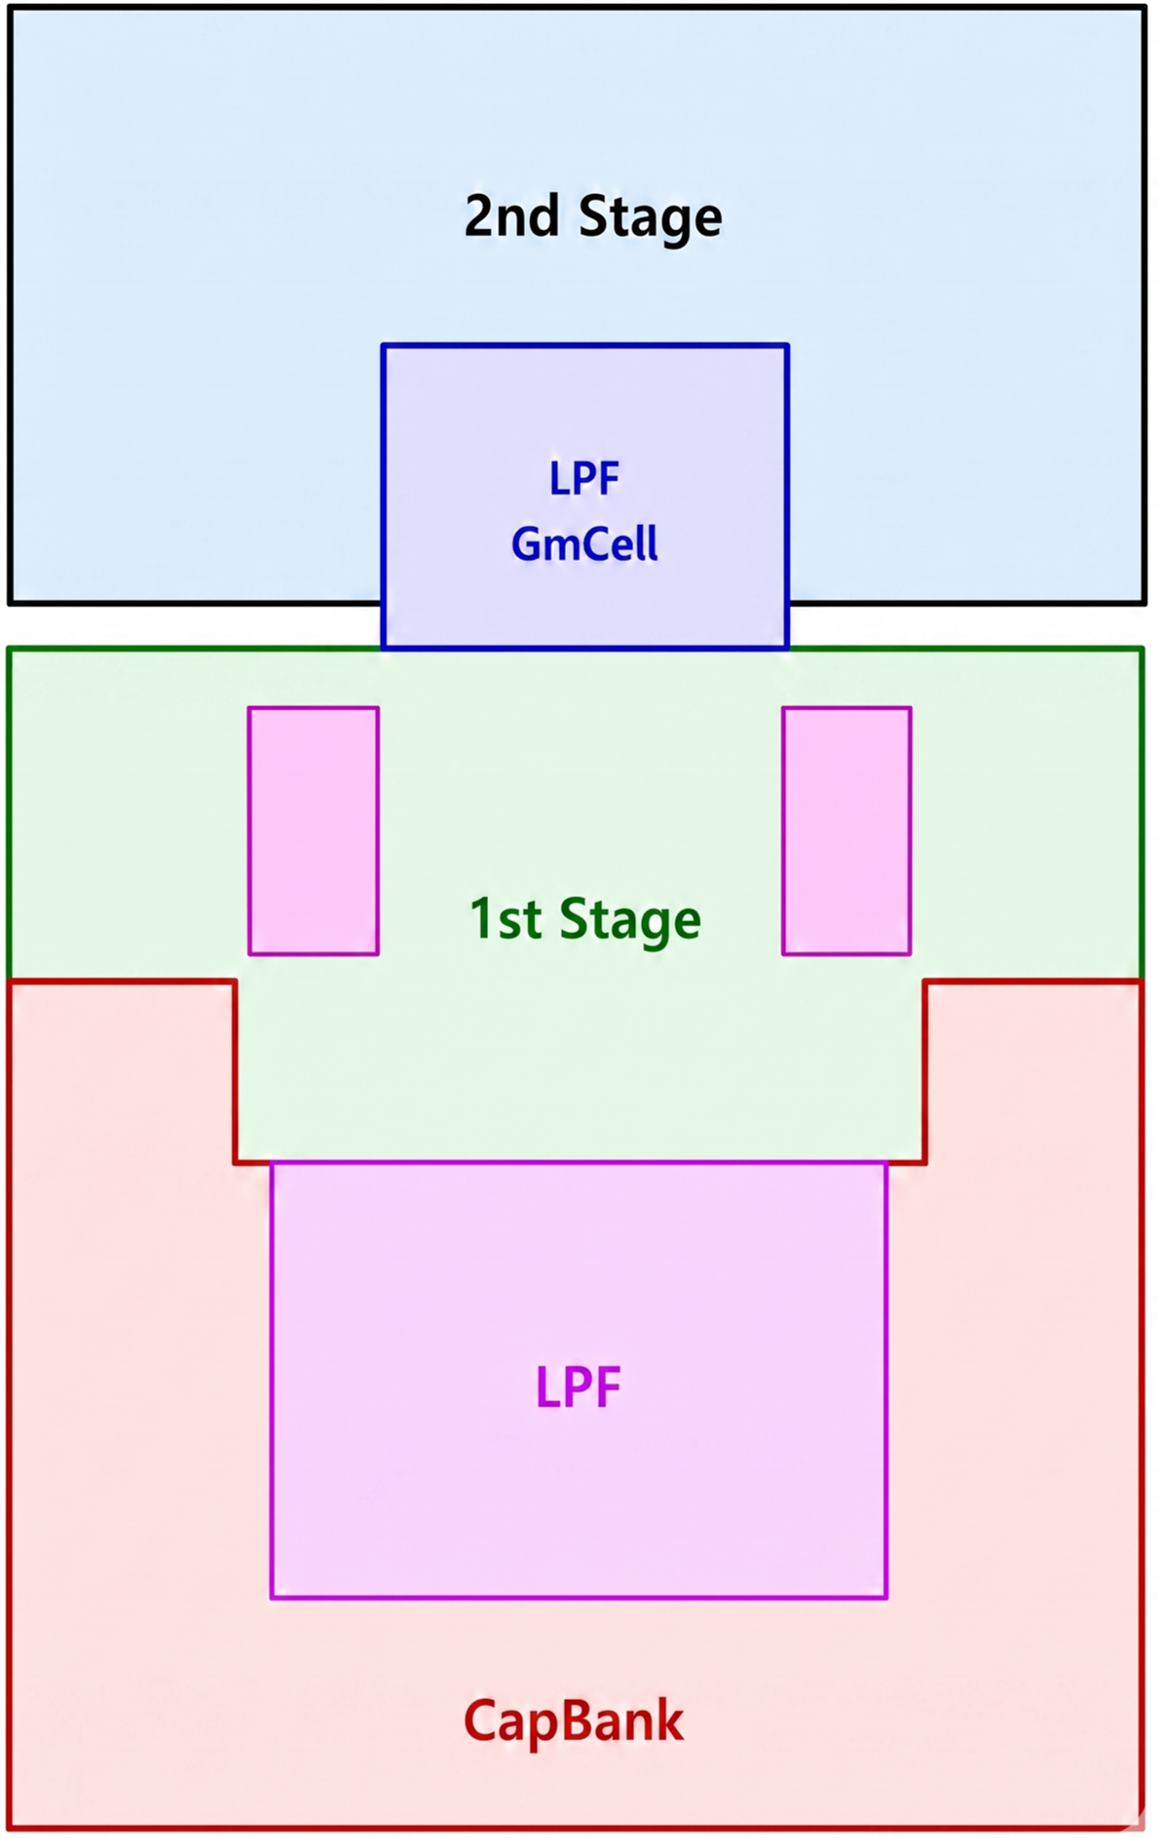
\includegraphics[width=\linewidth]{img/CTLE_img/ctle_floorplane_diagram.png}
    \end{minipage}\hfill
    \begin{minipage}{0.48\textwidth}
        \centering
        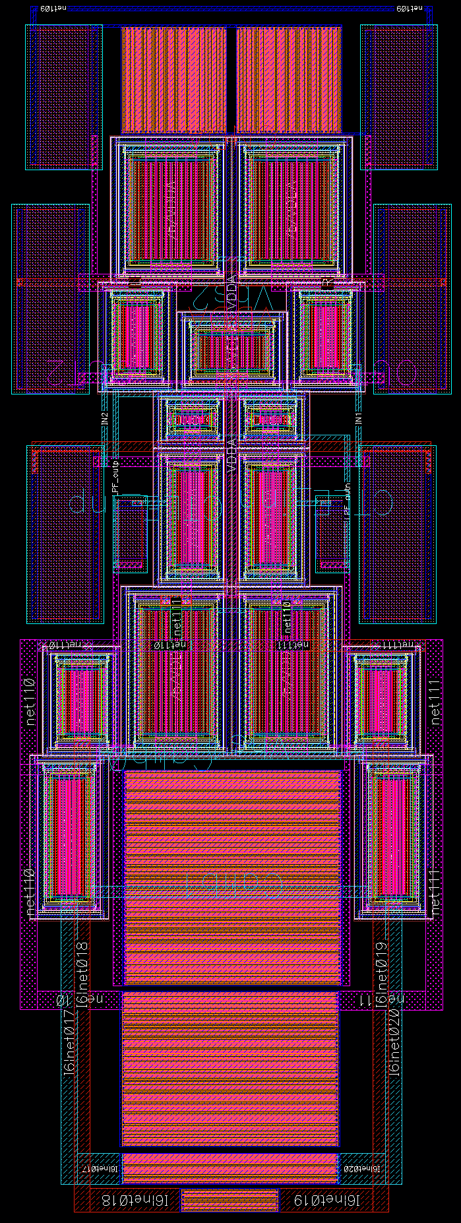
\includegraphics[width=0.7\linewidth]{img/CTLE_img/full_layout_without_Rbank.png}
    \end{minipage}
    \caption{Left: floorplan diagram illustrating the symmetric block-level arrangement. Right: Corresponding physical layout of the CTLE core (excluding the resistive bank), demonstrating the matched differential routing and component placement.}
    \label{fig:layout_floorplan}
\end{figure}

\newpage \noindent To complete the macro, the programmable thermometer-coded resistive bank (R-bank) is integrated alongside the core. Figure~\ref{fig:full_layout_with_Rbank} displays the complete top-level layout. The R-bank is placed adjacent to the 1st Stage source nodes to modularize the gain control while keeping the sensitive source degeneration routing as short and symmetric as possible.

\begin{figure}[H]
    \centering
    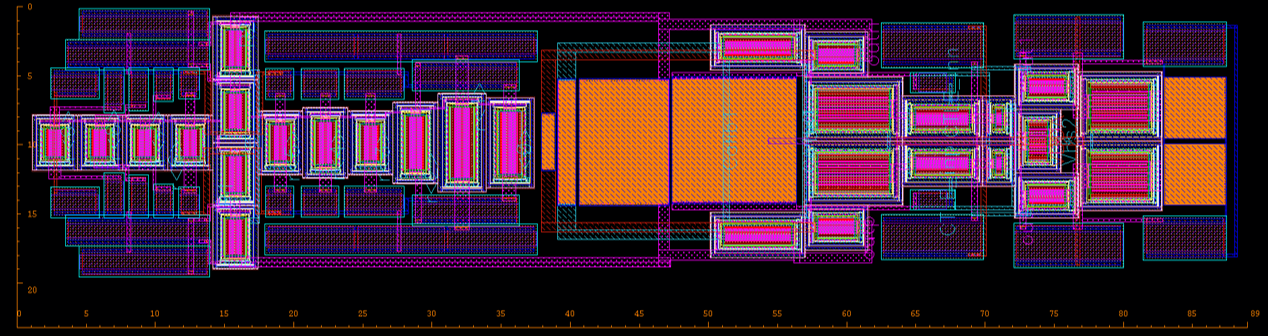
\includegraphics[width=0.95\textwidth]{img/CTLE_img/full_layout_with_Rbank.png}
    \caption{Complete physical layout of the CTLE macro. The thermometer-coded resistive degeneration bank is integrated on the left side, seamlessly connecting to the core differential pair's source nodes.}
    \label{fig:full_layout_with_Rbank}
\end{figure}

\subsubsection{Post-Layout Extraction (PEX) Simulation}

To validate the robustness of the physical design, Post-Layout Extraction (PEX) was performed to account for parasitic resistances and capacitances (RC) introduced by the metal routing, vias, and device proximities. Figure~\ref{fig:ctle_pex} compares the AC frequency response of the ideal pre-layout schematic against the fully extracted PEX netlist at the maximum boost setting (DC gain target of -15\,dB).

\begin{figure}[H]
    \centering
    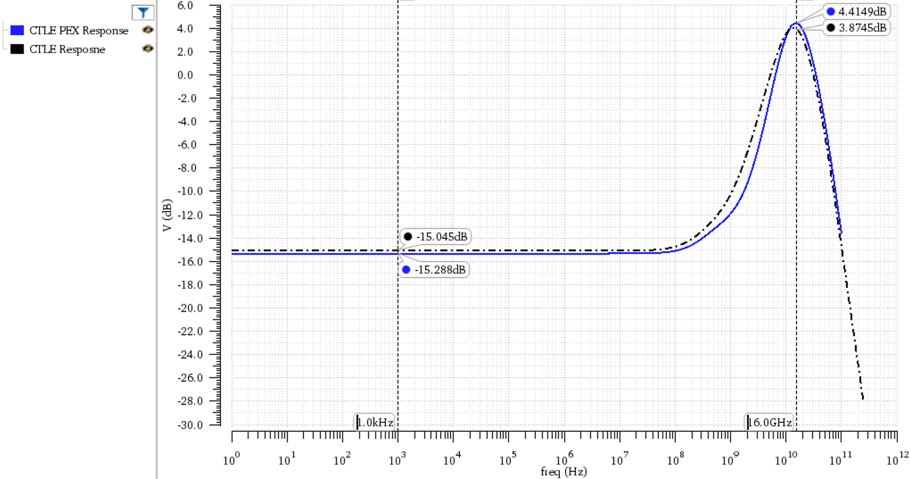
\includegraphics[width=0.90\textwidth]{img/CTLE_img/ctle_pex.png}
    \caption{AC response comparison between the pre-layout schematic simulation (dashed black) and the Post-Layout Extraction (PEX) simulation (solid blue) at the maximum boost configuration.}
    \label{fig:ctle_pex}
\end{figure}

\newpage
The PEX simulation results confirm that the layout successfully preserves the equalizer's core frequency characteristics with minimal degradation. The key comparative metrics extracted from the plot are:
\begin{itemize}[noitemsep]
    \item \textbf{DC Gain Drop:} The low-frequency DC gain experiences a negligible drop from -15.045\,dB (pre-layout) to -15.288\,dB (PEX). This minimal difference of $\approx 0.24$\,dB is attributed to the finite series resistance of the routing metal in the signal and bias paths.
    \item \textbf{High-Frequency Peaking:} The high-frequency peaking magnitude shows a slight enhancement, shifting from 3.87\,dB to 4.41\,dB near the 16\,GHz Nyquist frequency. This alteration in the zero-pole profile is primarily driven by the parasitic capacitance at the source degeneration nodes interacting with the layout traces.
\end{itemize}

Overall, the PEX validation demonstrates that the layout is highly optimized. The slight deviations induced by layout parasitics remain strictly within the acceptable calibration margins of the programmable C-bank and R-bank, ensuring the design will reliably meet PCIe 6.0 equalization targets post-fabrication.



\newpage
\subsection{Design Summary}
\label{sec:summary}

\subsection*{Specification vs. Achieved Performance}

Table~\ref{tab:summary} summarizes the target design specifications alongside the measured performance metrics for the complete two-stage CTLE. To rigorously validate the design's robustness and reliability, the values reported in the ``Achieved'' column represent the worst-case performance extracted across all simulated Process, Voltage, and Temperature (PVT) corners. 

\begin{table}[H]
    \centering
    \caption{Design summary: target specifications versus worst-case achieved performance.}
    \label{tab:summary}
    \begin{tabular}{lccc}
        \toprule
        \textbf{Parameter}         & \textbf{Spec}           & \textbf{Achieved (Worst-Case)} & \textbf{Status}         \\
        \midrule
        Supply voltage             & $0.8\,\text{V} \pm 5\%$ & $0.8\,\text{V} \pm 5\%$   & \textcolor{green!60!black}{\textbf{Pass}} \\
        DC gain range              & $-5$ to $-15$\,dB       & $-4.7$ to $-16.3$\,dB           & \textcolor{green!60!black}{\textbf{Pass}} \\
        DC gain step size          & 1\,dB                   & 1\,dB                      & \textcolor{green!60!black}{\textbf{Pass}} \\
        Boost range                & 9 to 19\,dB             & 8 to 20\,dB               & \textcolor{green!60!black}{\textbf{Pass}} \\
        Output-referred noise      & ---                     & $767.6\,\mu\text{V}_{\text{rms}}$ & --- \\
        Output swing               & ---                     & $210\,\text{mV}_{\text{pp,diff}}$       & --- \\
        Input swing (@$-15$\,dB)   & ---                     & $1.1\,\text{V}_{\text{pp,diff}}$        & --- \\
        Input swing (@$-5$\,dB)    & ---                     & $660\,\text{mV}_{\text{pp,diff}}$       & --- \\
        Silicon area               & Not specified           & $89\times 20\,\mu\text{m}^2$ & --- \\
        Max current                & $<20$\,mA               & $13.16\,\text{mA}$             & \textcolor{green!60!black}{\textbf{Pass}} \\
        Temperature range          & $-40$ to $125\,^{\circ}$C & $-40$ to $125\,^{\circ}$C & \textcolor{green!60!black}{\textbf{Pass}} \\
        \bottomrule
    \end{tabular}
\end{table}
